% Chapter Template

\chapter{History of age--activity--rotation relationships} % Main chapter title

\label{Chapter2} % Change X to a consecutive number; for referencing this chapter elsewhere, use \ref{ChapterX}

%----------------------------------------------------------------------------------------
%	SECTION 1
%----------------------------------------------------------------------------------------

\epigraph{\itshape The past can hurt. But the way I see it, you can either run from it or learn from it.}{---Rafiki, \textit{The Lion King}}

\section{Introduction}

The history of age--activity--rotation studies dates back to the 1960's, when the theoretical framework for these relationships (i.e. magnetic braking) was first theorised by \citet{Schatzman_1962}. \citet{Wilson_1963} first suggested that emission in \caII lines (and chromospheric activity in general) declined with stellar age. This was based off observations that the average intensity of \caII emission was much higher for main-sequence stars in several clusters (including Hyades and Praesepe) than for local field stars. \citet{Kraft_1967} suggested the same concerning rotation based off a sample of rotational velocities ($vsin(i)$) for a large sample of field stars with the average rotational velocity being higher for stars with \caII emission than those without. Since there was evidence that the \caII emission declined with age then so must the rotational velocity.

Probably the most cited paper concerning activity, rotation and their evolution in time is the seminal paper by \citet{Skumanich_1972}. This paper was the first to plot activity and rotation as a function of age using data from the Pleiades, Ursa Major, Hyades and the Sun as shown in Figure \ref{fig:Skumanich_plot}. Skumanich found that the calcium emission and rotational velocities followed a power law: $Ca^{+} \propto \tau^{-\frac{1}{2}}$ where $\tau$ is the stellar age. This power law is commonly known as the Skumanich Law and modern studies still compare results to this relationship. The rest of this chapter will highlight some of the most relevant papers that document the progress of the age--activity--rotation relation, what has been achieved and what can still be improved upon.

\begin{figure}
    \centering
    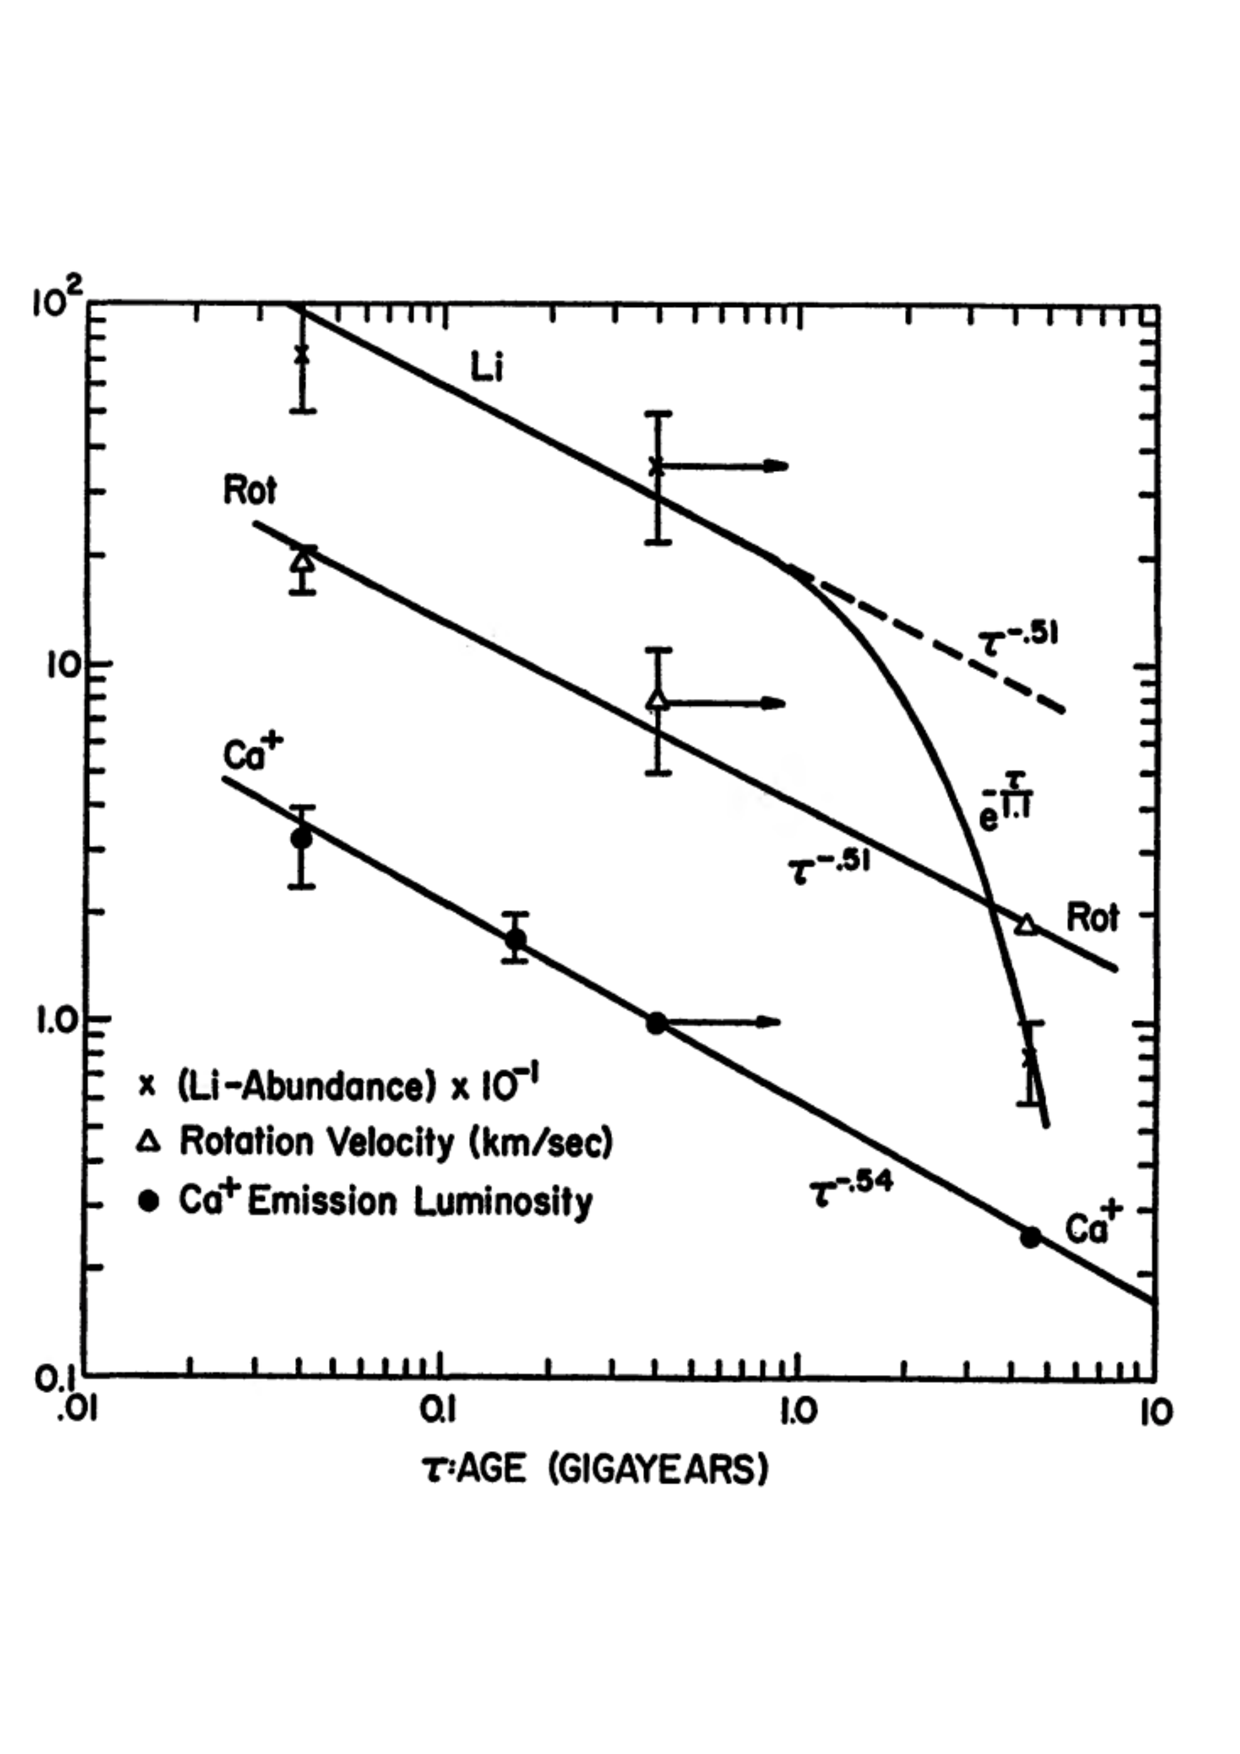
\includegraphics[scale=0.45]{Figures/2-Historical_overview/skumanich_1972.pdf}
    \caption[First plot of age-activity--rotation relationship]{Calcium emission, lithium abundance and rotational velocity as a function of age for two clusters and the Sun. The solid lines represent the Skumanich law - $\propto \tau^{-\frac{1}{2}}$ Image credit: \citet{Skumanich_1972}}
    \label{fig:Skumanich_plot}
\end{figure}

\section{Age--rotation studies (Gyrochronology)}
The term generally used to denote the age--rotation relationship is "gyrochronology" which originates from the seminal paper by \citet{Barnes_2003}. The general relationship between the rotational velocity and age can be written as shown in Equation \ref{Eq:general_rotation_age}, this will become important for Section \ref{Chp2_section_activity_age}.

\begin{equation}
    v_{rot} \propto t^{\alpha}
    \label{Eq:general_rotation_age}
\end{equation}

\citet{Barnes_2003} gathered rotation periods for a number of open clusters alongside old Mount Wilson stars allowing for a wide variety of stars to be studied together. The rotation periods for each cluster/group are plotted as a function of (B-V) colour as shown in Figure \ref{fig:barnes_2003_plot}. From these plots, \citet{Barnes_2003} was able to identify several sequences with the most important two for this discussion being the I and C sequence, later termed the Interface and Convective sequences (pertaining to the type of dynamo present, see \citet{Barnes_2003} for a full discussion).

\begin{figure}
    \centering
    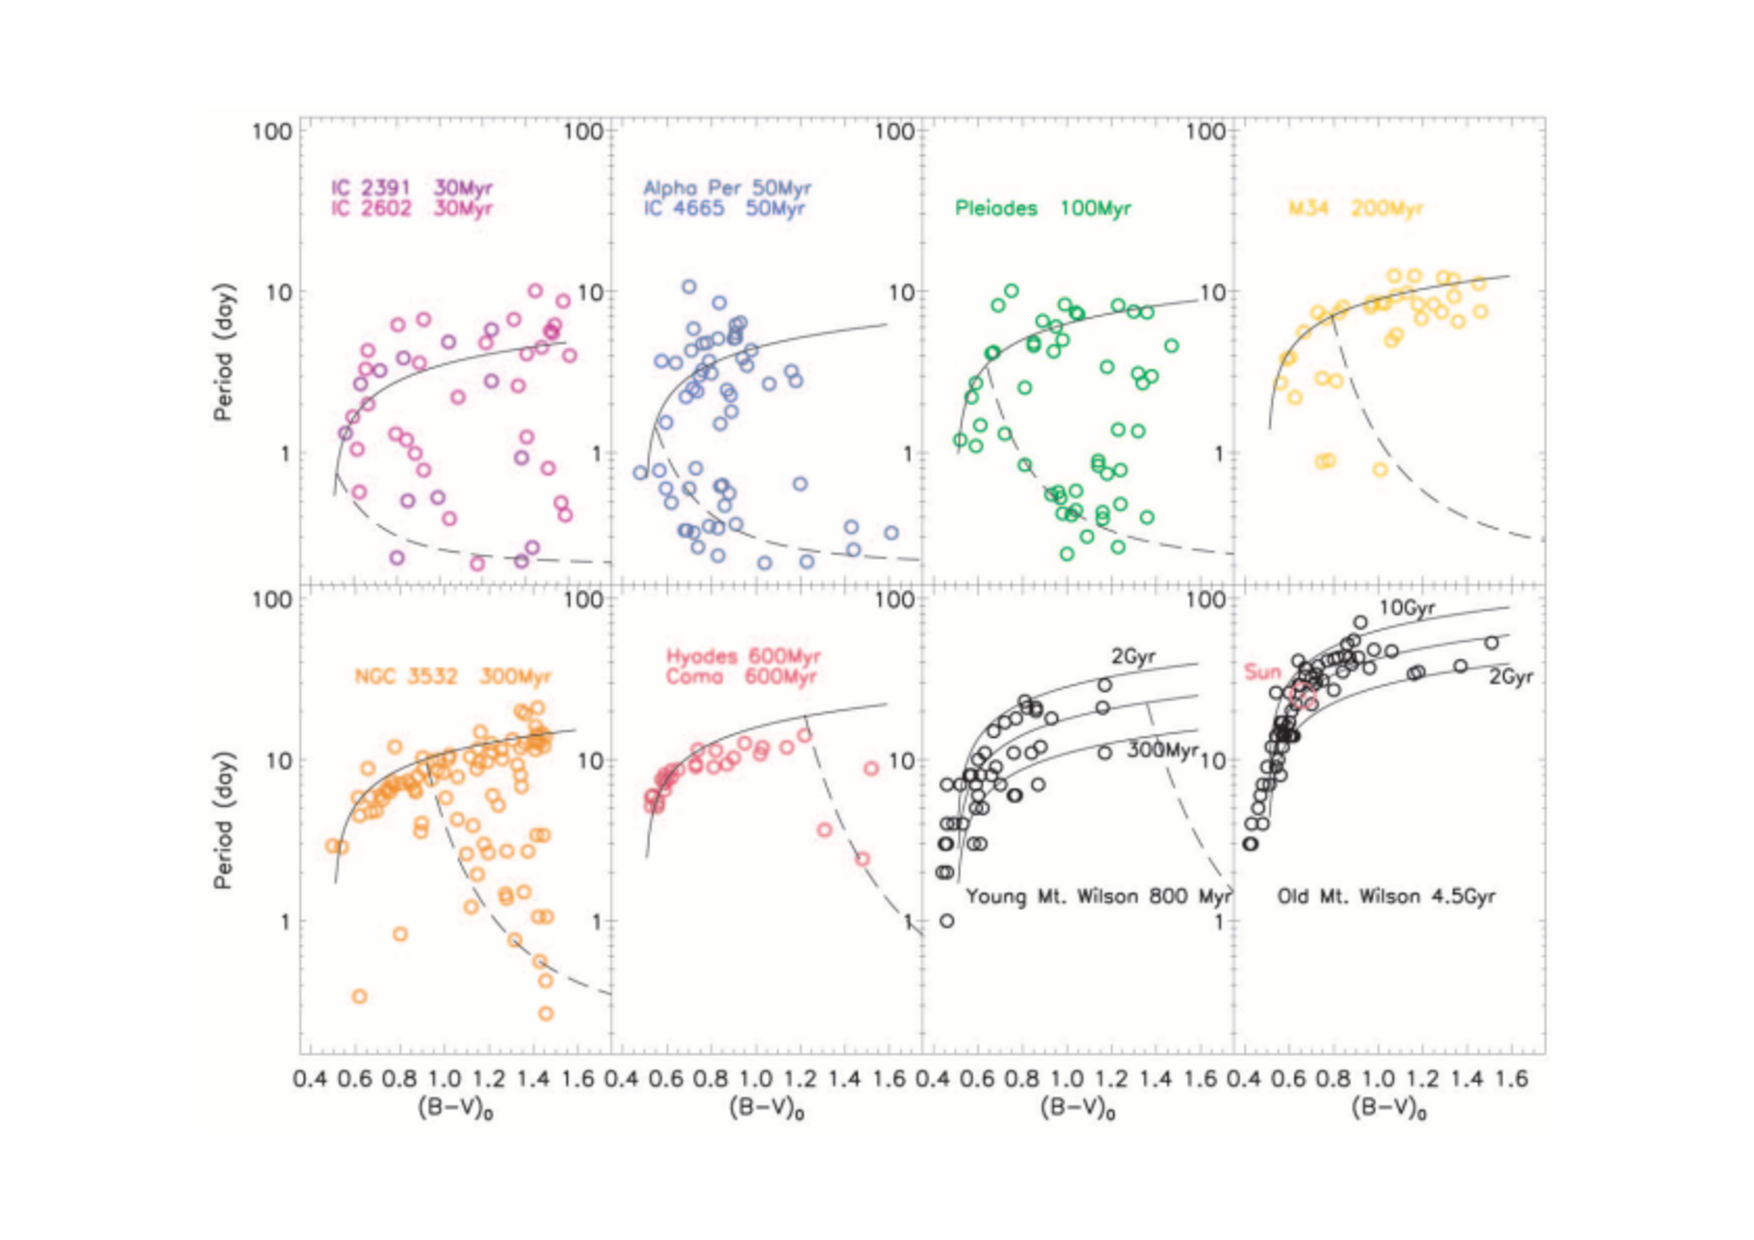
\includegraphics[scale=0.5]{Figures/2-Historical_overview/barnes_2003.pdf}
    \caption[Rotation period as function of colour for a number of clusters]{Plot of rotation period as a function of (B-V) colour for a number of clusters and a sample of Mount Wilson stars which are divided up into young and old ages. Dashed lines indicate the position of the I and C sequences (see text for details).}
    \label{fig:barnes_2003_plot}
\end{figure}

The I sequence is a diagonal band of increasing period with increasing (B-V) colour which is only faintly visible in the youngest cluster but becomes more pronounced as one proceeds to older ages. It also accounts for an increasingly large fraction of stars as in the Hyades cluster all but three stars lie on this sequence and the sequence makes up the whole sample when considering the Mount Wilson sample. The positive slope of this sequence also increases with stellar age indicating that lower mass stars spin down faster and higher mass stars spin down slower or hardly at all.

In the youngest clusters, a sequence of ultra-fast rotators (UFR's) are also observed and known as the C sequence. This sequence bifurcates away form the I sequence towards shorter rotation periods. Initially this sequence is well populated but becomes increasingly sparse with age, it also seems to be lifted with time towards longer rotation periods. \citet{Barnes_2003} noted that the C sequence never crosses the I sequence but the point at which it starts bifurcating from the I sequence moves to redder values of (B-V) colour with age. The decreasing population of the C sequence also suggests that stars move from the C to I sequence over time. The region between the two sequences is known as the gap and is also often populated. However, this is more sparsely populated than the other two sequences. It's population density also decreases with age. This also fits in with the theory that stars move from the C to I sequence.

\citet{Barnes_2003} also determined a formula for using rotation as an age indicator once stars have converged onto the I sequence. This formula shown in Equation \ref{Eq:B03_eq_1} shows that the rotation period is both dependent on the age of the star and the colour; note that this relationship is consistent with the Skumanich law. Equation \ref{Eq:B03_eq_2} shows the dependence on the colour parameter. If these equations are plotted for a given age and a range of colours, this results in a rotational isochrone, opening up the possibility of dating clusters by looking at fundamental parameters.

\begin{equation}
    P_{rot} = \sqrt{t}f(B-V)
    \label{Eq:B03_eq_1}
\end{equation}

\begin{equation}
    f(B-V) = \sqrt{(B-V) -0.5} - 0.15(B-V-0.5)
    \label{Eq:B03_eq_2}
\end{equation}

Further work was conducted by \citet{Barnes_2007} to improve the gyrochronology relationship in order to determine ages for field stars. They derived a formula using open clusters ranging from 30 - 600 Myr in age. The clusters enabled the mass dependency to be determined to a higher accuracy as they contain a large range of masses for a given age; the mass dependency found by \citet{Barnes_2007} is given by Equation \ref{Eq:B07_mass_eq}.

\begin{equation}
    f(B-V) = 0.7725(B-V-0.4)^{0.601}
    \label{Eq:B07_mass_eq}
\end{equation}

The age dependence was based off the solar value as it has the best known rotation period. The solar values for rotation period, age and (B-V) colour were used to determine the exponent of the age dependency shown in Equation \ref{Eq:B07_age_eq}. Therefore to determine the rotation period for a star of a given age and colour Equation \ref{Eq:B07_combine_eq} could be used. \citet{Barnes_2007} derived errors for ages and found that these were typically $\sim 15$\% not including systematics.

\begin{equation}
   g(t) = t^{0.5189}
    \label{Eq:B07_age_eq}
\end{equation}

\begin{equation}
    P(B-V, t) = f(B-V)g(t)
    \label{Eq:B07_combine_eq}
\end{equation}

In order to test these updated relations derived in \citet{Barnes_2007}, a comparison was made to chromospheric ages which showed good agreement. Ages were also calculated for individual members of binary systems and they found that the binary members showed the same age giving confidence to the relations determined in the paper.

However, more clusters were needed to confirm the existing gyrochronology relationships. One notable breakthrough in this regard was the study of the 2.5 Gyr old cluster NGC 6819 by \citet{Meibom_etal_2015}. A sample of 30 cool stars ranging from 0.85 to 1.4 solar masses with rotation periods determined from Lomb-Scargle periodograms of long-cadence Kepler data were analysed. The data for this cluster was plotted alongside previous cluster data (as shown in Figure \ref{fig:Meibom_etal_2015_plot}) and found to agree with previous gyrochronology relationships. This study bridged a gap in observational data between the Hyades cluster and solar values and provided confirmation in existing gyrochronology relationships.

\begin{figure}
    \centering
    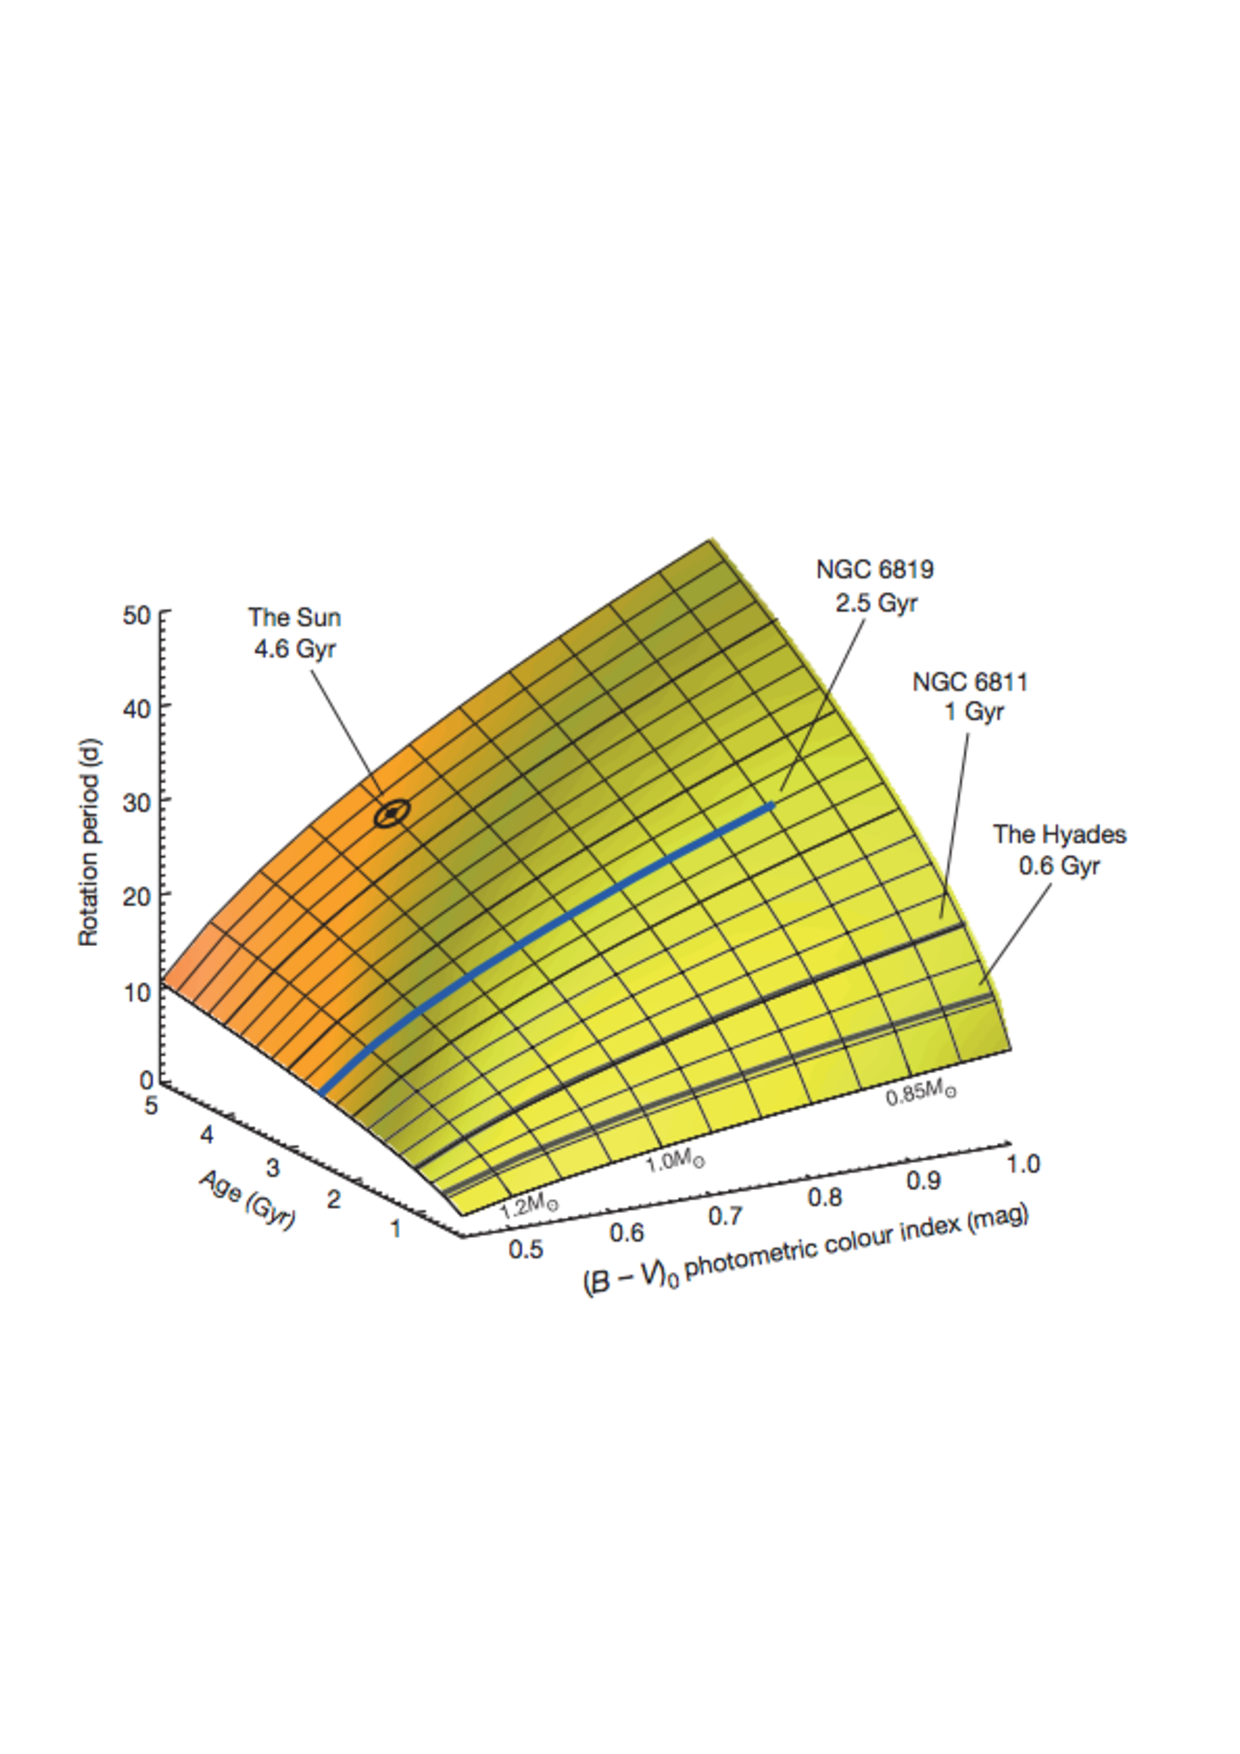
\includegraphics[scale=0.55]{Figures/2-Historical_overview/meibom_etal_2015.pdf}
    \caption[Comparison of data from 2.5 Gyr old cluster to previous gyrochronology relationship]{Observations of rotation periods from NGC 6819 alongside younger clusters and solar values. Yellow surface represents the typical gyrochronology relationship which shows good agreement with the cluster data. Image credit: \citet{Meibom_etal_2015}}
    \label{fig:Meibom_etal_2015_plot}
\end{figure}

At this stage in the literature, the cluster observations seemed to be confirming that if the mass (or colour) of the star is taken into consideration then the rotation period could be used to date the star. But with the launch of Kepler, the field of asteroseismology had been rapidly expanded to detect even more solar-like oscillators for which ages could be determined for \citep{Chaplin_etal_2011}. The first attempt at extending gyrochronology to older ages by considering asteroseismic ages was by \citet{Angus_etal_2015}.

This study considered 310 Kepler stars with asteroseismic ages, 50 stars from the Hyades and Coma Berenices clusters and 6 field stars with precise ages (including the Sun). \citet{Angus_etal_2015} calibrated a relation in the form shown in Equation \ref{Eq:Angus_etal_2015_eq} where A is the age in Myr and the free parameters fitted are a, b, c and n. The best-fitting values for these parameters were: a=0.40, b-0.31, c=0.45 and n=0.55.

\begin{equation}
    P = A^{n}a(B - V - c)^{b}
    \label{Eq:Angus_etal_2015_eq}
\end{equation}

\citet{Angus_etal_2015} also investigated the posterior probability distribution function of the gyrochronology parameters, including an analysis of different subsets of the data. This analysis found tension between the asteroseismic ages and the gyrochronology relation as no single relation could adequately describe all subsets of the data. this provided concerns over the use of gyrochronology as an age dating method. It is worth noting that the asteroseismic ages used in \citet{Angus_etal_2015} were calculated from global modelling of the asteroseismic parameters which are known to be more uncertain than when individual frequencies are modelled.

\begin{figure}
    \centering
    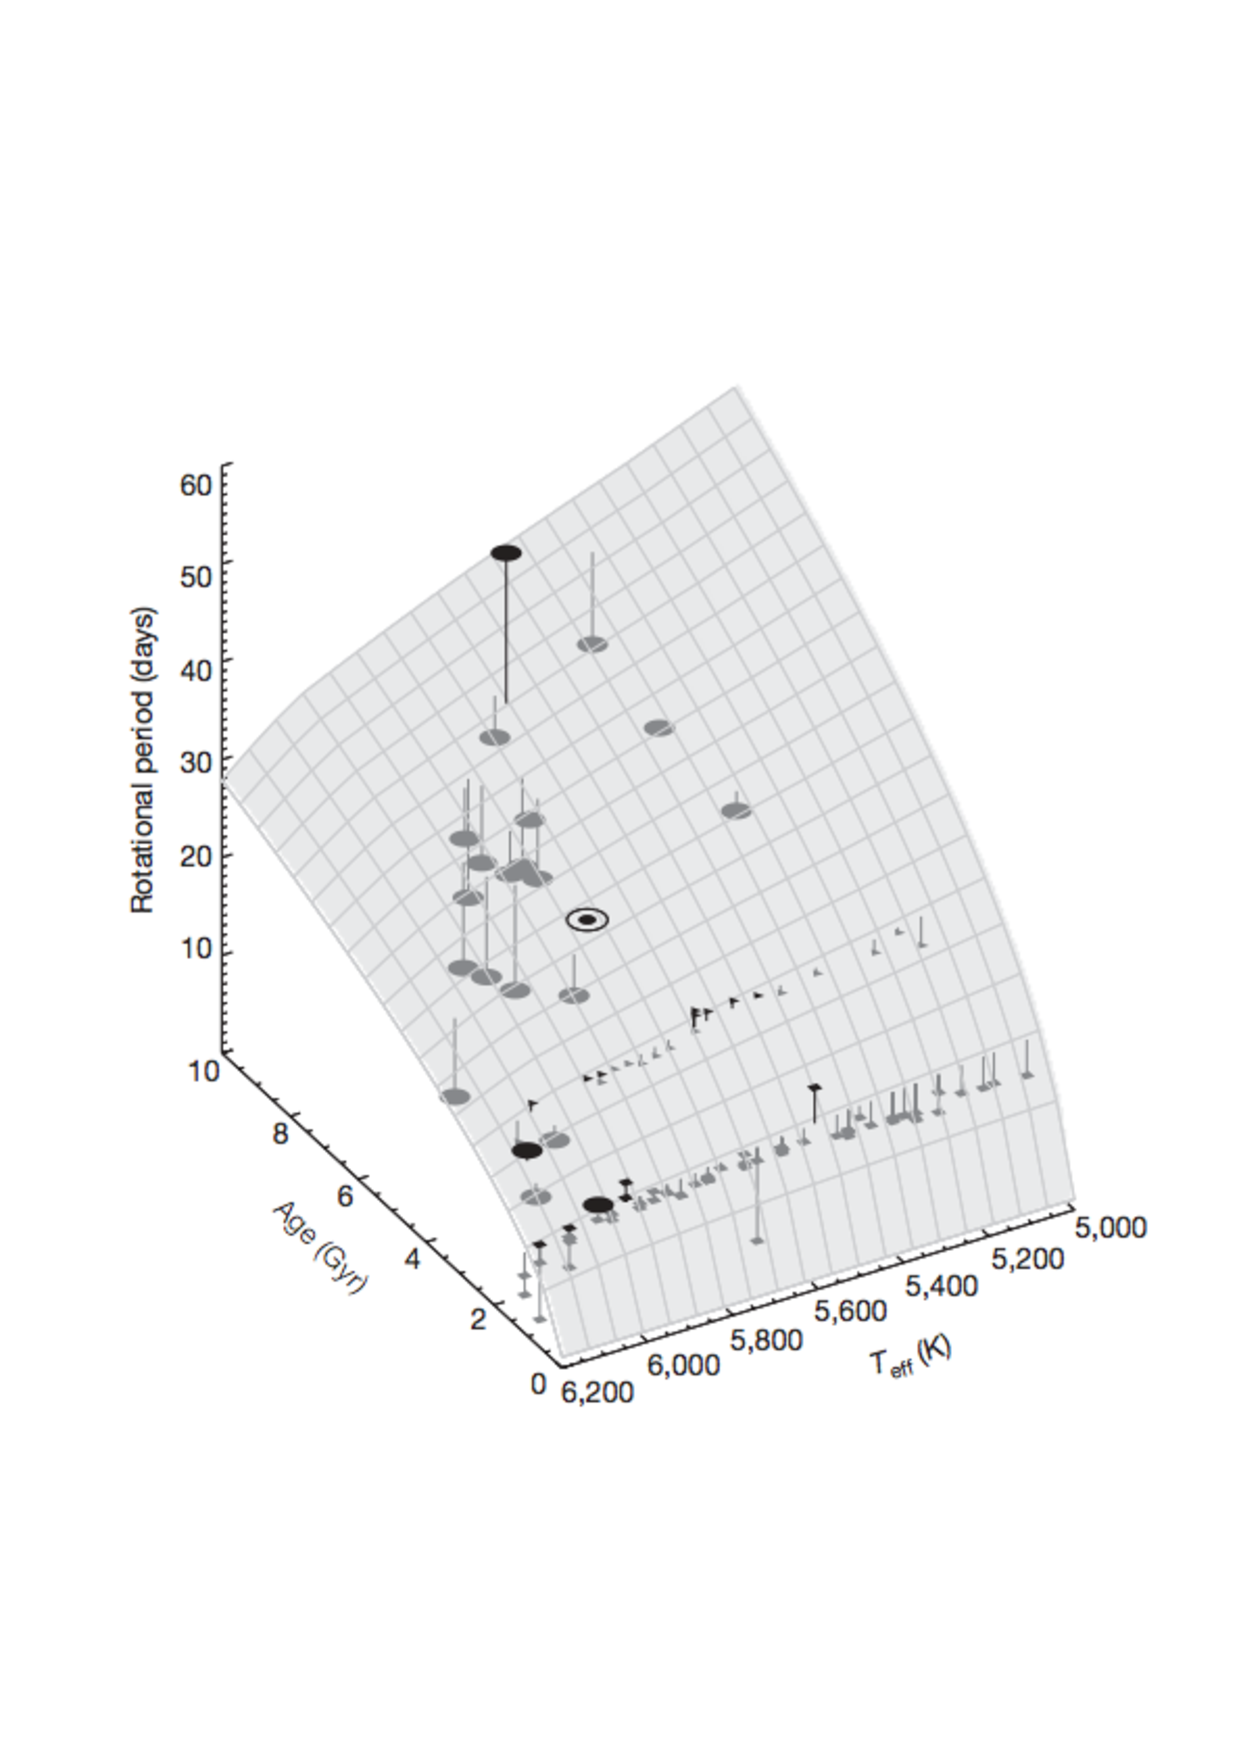
\includegraphics[scale=0.45]{Figures/2-Historical_overview/van_saders_3d_plot.pdf}
    \caption[Comparison of older sample of stars to previous gyrochronology relaitonship and cluster data]{Plot of rotation period, effective temperature and age for \citet{van_Saders_etal_2016} sample alongside cluster data. An empirical relationship is also shown. Image credit: \citet{van_Saders_etal_2016}}
    \label{fig:van_saders_plot_1}
\end{figure}

\begin{figure}[h]
    \centering
    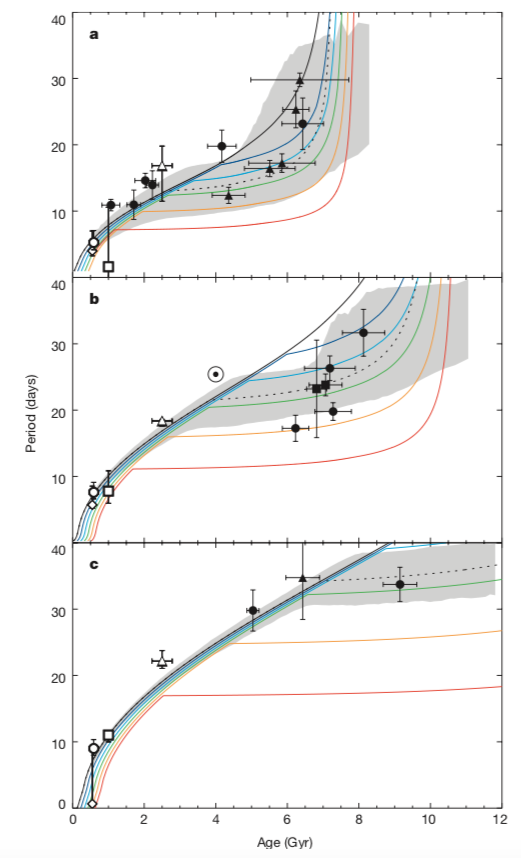
\includegraphics[scale=0.35]{Figures/2-Historical_overview/van_saders_R0_plot.png}
    \caption[Rotation period as a function of age with various stellar models that include a critical Rossby number]{Plot of rotation period as a function of age  for \citet{van_Saders_etal_2016} sample alongside cluster data divided into three effective temperature ranges from hottest in the top (a) panel and coolest in bottom (c) panel. Curves represent various stellar models with different critical Rossby numbers ranging from 0 (black line) to 3.0 (red). Dashed line shows best fit for critical Rossby number of $R_{0} = 2.16$. Image credit: \citet{van_Saders_etal_2016}}
    \label{fig:van_saders_plot_2}
\end{figure}

\begin{figure}[h]
    \centering
    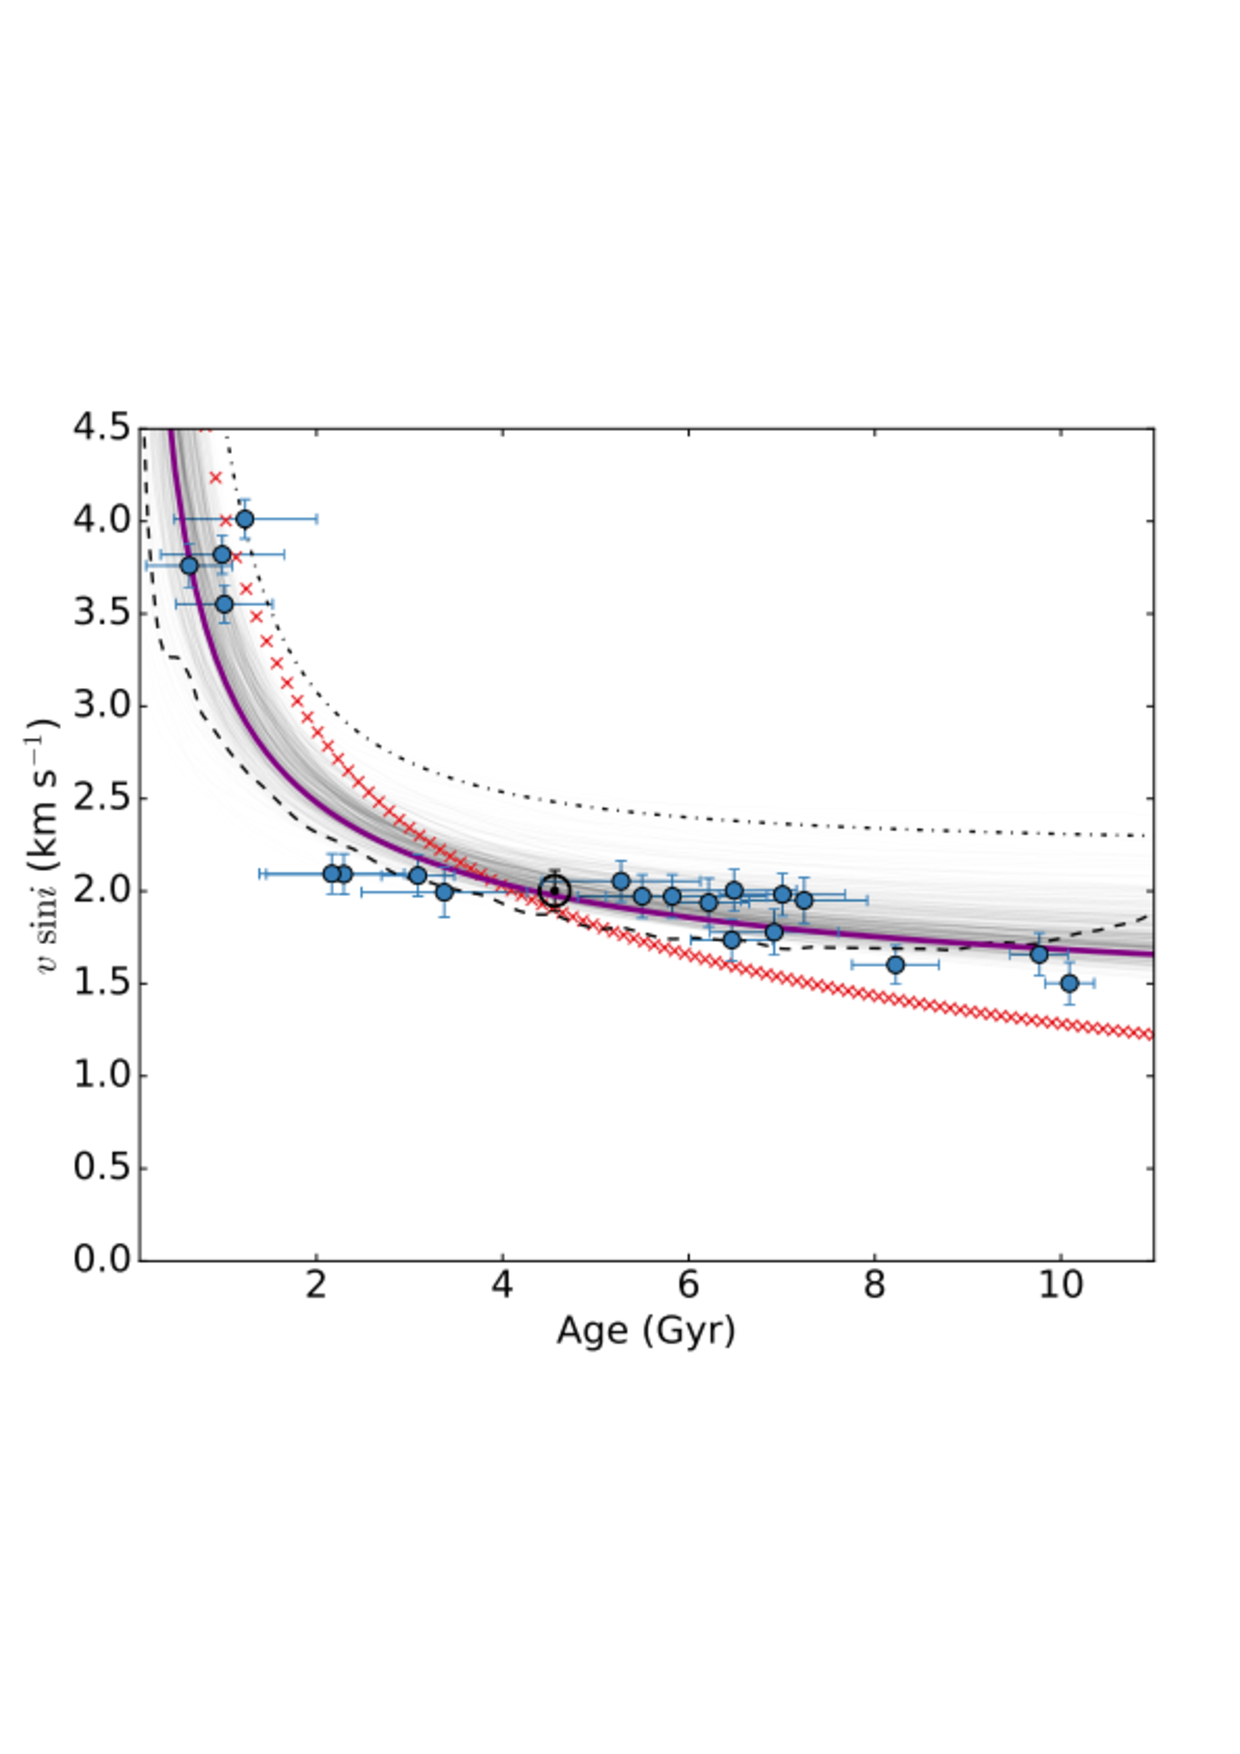
\includegraphics[scale=0.35]{Figures/2-Historical_overview/dos_santos_2016.pdf}
    \caption[Rotational evolution of sample of solar twins from \citet{dos_Santos_etal_2016} ]{Plot of selected sample of solar twins from \citet{dos_Santos_etal_2016} with projected rotational velocity as a function of age.The purple line represents the best-fitting relationship found for this sample ($v \propto t^{-0.6}$). The red crosses represents the Skumanich Law, the black dashed curve represents the \citet{do_Nascimento_etal_2014} relationship and the black dot-dashed curve represents the relationship from \citet{Pace_Pasquini_2004}. Image credit: \citet{dos_Santos_etal_2016}}
    \label{fig:dos_santos_2016}
\end{figure}

The tension between asteroseismic ages and gyrochronology increased when \citet{van_Saders_etal_2016} presented a sample of field stars with precise asteroseismic ages from individual frequency modelling. Their sample consisted of 21 Kepler stars with high precision ages, rotation periods from photometric variability and measured metallicities. Figure \ref{fig:van_saders_plot_1} shows the empirical gyrochronology relationship and the observed rotation periods for the \citet{van_Saders_etal_2016} sample of stars, they found that the majority of their sample of stars lay below the empirical surface. They found that stars more evolved than the Sun showed rapid rotation which persisted across a range of effective temperatures and they interpreted this as weakened magnetic braking.

\citet{van_Saders_etal_2016} postulated that above a critical value the effective loss of angular momentum stopped; this critical value was considered in term of Rossby Number. The Rossby number ($R_{0}$) is defined as the rotation period divided by the convective turnover time ($\tau_{c}$) and is commonly used in the activity--rotation relationship (see Section \ref{Chp2_activity-rotation_lit_review}). The convective turnover time is defined as the typical timescale taken for a convective cell to rise and is dependent on the mass of the star as this is the main parameter that determines the depth of the convection zone. To test this hypothesis, \citet{van_Saders_etal_2016} modified stellar models to conserve angular momentum above a certain critical $R_{0}$. Figure \ref{fig:van_saders_plot_2} shows cluster data and the sample of older stars with various stellar angular momentum models with the inclusion of the critical Rossby number. \citet{van_Saders_etal_2016} find the best critical Rossby number is 2.16 which is able to explain both the the young cluster data and old sample of stars. This results cast doubt on the use of rotation period as an age indicator as it may only work for part of the stellar population. Note that the age at which the gyrochronology relation is no longer valid, according to this result, is different for varying stellar masses. The data in panel (b) of Figure \ref{fig:van_saders_plot_2} would suggest that the Sun is on the cusp of the transition to weakened magnetic braking.

Further evidence for a modified braking law for solar-like stars was presented by \citet{dos_Santos_etal_2016}. The work found the projected rotational velocities for a sample of 81 solar twins by using high resolution spectra from \textit{HARPS} and fitting with synthetic spectra. Ages for this sample of stars were determined using isochrones. Since the projected rotational velocity is dependent on the inclination of the star, to investigate the rotational evolution using this parameter, \citet{dos_Santos_etal_2016} determined a subset of their data called the 'selected sample'. This sample was determined by removing the spectroscopic binaries and dividing the rest of the sample into age bins of 2~Gyr. In each bin, they removed stars that were below the 70\ts{th} percentile of the projected rotational velocity. This was justified through a simulation with angles $i$ drawn from a flat distribution between $0$ and $\pi/2$ that showed 30~\% of stars should have a value of $v\sin(i)$ greater than 0.9. This selected sample of 21 stars and the Sun were used to calibrate the relationship between rotation and age. An orthogonal distance regression (ODR) was used to calibrate the relationships as this accounts for errors in both sets of parameters. \citet{dos_Santos_etal_2016} found that a rotational braking law of $v \propto t^{-0.6}$ was the best fitting relationship for their sample of solar twins. Figure \ref{fig:dos_santos_2016} shows the age--rotation plot for the selected sample of stars along with the best fitting relationship and several other age--rotation relationships. The discrepancy seen between the Skumanich law and the solar twin sample is most prominent after the solar age. They propose a new rotational braking law that supports the weakened braking after the age of the Sun, similar to the conclusion \citet{van_Saders_etal_2016} made.

Despite the tension between gyrochronology and asteroseismic ages, research continued to extend the relationship using clusters. \citet{Barnes_etal_2016} reported rotation periods for 20 cool (FGK) stars in the 4 Gyr old M67 cluster with data from the K2 mission. Rotation periods were determined from the 75 day baseline data with four different methods. The authors do note that the length of the baseline is long enough for starspot evolution but not long enough for multiple phases of periodic variations due to starspots.

\citet{Barnes_etal_2016} plotted the rotation period as a function of (B-V) colour and saw a similar shape to that seen in younger clusters (see Figure \ref{fig:barnes_2003_plot} for shape). Therefore, they conclude that since M67 shows a cross section of the gyrochronology surface at an age of 4 Gyr, gyrochronology relations are valid to at least solar age. The study also calculated gyrochronology ages for the individual cluster members of M67 and found a standard deviation from the true cluster age of 0.7 Gyr which is equivalent to approximately 17\%. The authors suggest that similar errors could be achieved for ages of K2 planet hosts.

However, there are possible limitations to determining rotation periods for older clusters using data from K2. \citet{Esselstein_etal_2018} presented a sample of comprehensive injection tests into M67 light curves from the K2 campaign (i.e. the same data \citealt{Barnes_etal_2016} used) and they attempt to recover the injected signals with a Lomb-Scargle periodogram analysis. While they find that the reliability of the detected rotation periods are high, they also find that the sensitivity drops rapidly with increasing rotation period and decreasing amplitude. In the case of a solar rotator, they find that there is only a 15\% recovery rate. This study highlighted the need for caution when determining rotation periods for any cluster observed by K2 or similar missions such as TESS.

In \citet{Barnes_etal_2016_aspect_gyro}, the authors discuss the implications of the claimed weakened magnetic braking by \citet{van_Saders_etal_2016}. They claim that the transition at 2.5 Gyr (for stars with effective temperatures: $5900 < T_{eff} < 6200 K$) is ruled out due to the observations of M67 \citep{Barnes_etal_2016} that obey previous gyrochronology laws. However, one could also argue that \citet{Barnes_etal_2016} only had two stars within a similar colour range; this result based on two data points is not statistically significant, perhaps more data is needed to confirm this argument.

\citet{Barnes_etal_2016_aspect_gyro} also argue that other factors could be at fault for the sudden change in rotation periods at older ages and that it may not be a change in the angular momentum evolution. They considered the sample used in \citet{van_Saders_etal_2016} and removed several stars from the sample including stars with $\log(g) < 4.2$ which are post-turnoff stars. They also removed four metal poor stars and 16 Cyg A and B whose seismic rotation periods are incorrect (however, they do not state the reason why they are incorrect). For the remaining eight stars, they found that the gyrochronology ages (as calculated from \citealt{Barnes_2010}) and asteroseismic ages show good agreement.

More recently, \citet{van_Saders_etal_2019} have considered the challenges of interpreting large data sets such as the Kepler data set. In this study, they combine theoretical models of stellar rotation, stellar population model for the galaxy and prescriptions for observational biases to predict the rotational distribution in the Kepler field. The conclusions from the study were firstly that the standard breaking models fail to reproduce the observed distribution at long rotation periods and secondly, that the interpretation of the rotational distribution is complicated by mixtures of unevolved and evolved stars alongside observational uncertainties. \citet{van_Saders_etal_2019} define a threshold Rossby number of 2.08, this is the Rossby edge above which long period high Rossby number stars are either absent or undetected. Note that this value is comparable to the critical Rossby value of 2.16 found in \citet{van_Saders_etal_2016}. The authors conclude that either modified braking is in operation of the full Kepler population or stars undergo a transition in their starspot configuration at a similar Rossby number.

\section{Activity--rotation studies}
\label{Chp2_activity-rotation_lit_review}

From stellar dynamo theory (see Section \ref{Section:intro_dynamo_and_braking_section}), it is known that the stellar magnetic field (and thus magnetic activity) is linked to the rotation of the star through the dynamo effect. Hence it is expected that the magnetic activity and rotation period should be correlated in some way, this has led to several investigations of the activity--rotation relationship which shall be discussed in this section. The general expression for the activity--rotation relationship (in terms of X-ray luminosity) is shown in Equation \ref{Eq:general_activity_rotation}.

\begin{equation}
    L_{x} \propto P_{rot}^{\beta}
    \label{Eq:general_activity_rotation}
\end{equation}

The earliest study of this kind was conducted by \citet{Pallavicini_etal_1981} who analysed the relationship between X-ray luminosity and rotational velocities for stars of varying spectral types and luminosity classes using data from Einstein. In order to study the rotational aspect of the relationship, the study used rotational velocities as calculated from line broadening of spectral lines - $v\sin(i)$ where $v$ is the equatorial velocity and $i$ is the inclination angle. For late type stars (G-M), \citet{Pallavicini_etal_1981} plotted X-ray luminosity as a function of rotational velocities (as shown in Figure \ref{fig:pallavicini_etal_1981_plot}) and found the best fitting relationship as shown in Equation \ref{Eq:pallavicini_81}. The authors do emphasise that the data is still fairly scarce and that new high-sensitive data is needed but as we shall see from more recent studies, this relationship found by \citet{Pallavicini_etal_1981} holds up fairly well.

\begin{figure}
    \centering
    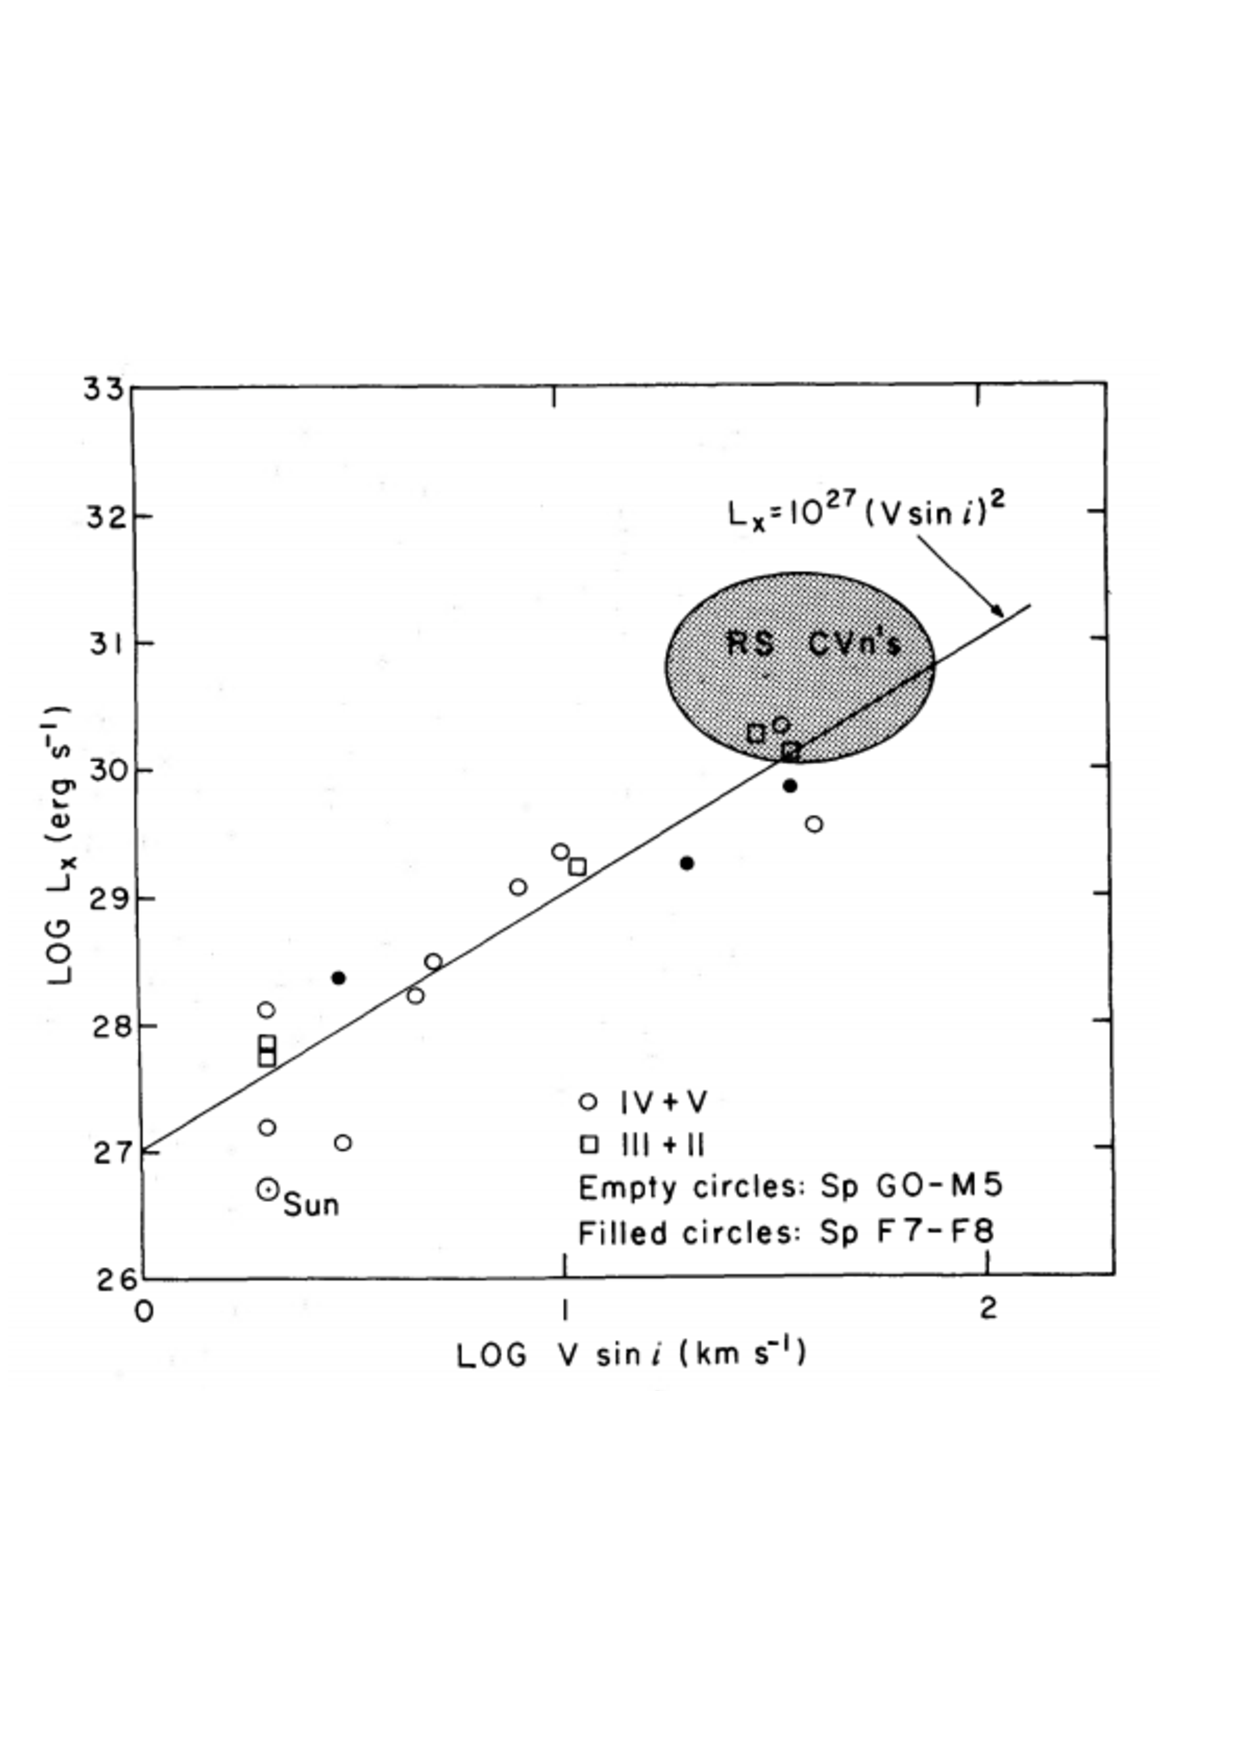
\includegraphics[scale=0.5]{Figures/2-Historical_overview/p81_fig_5.pdf}
    \caption[First plot of magnetic activity as a function of rotational velocity]{X-ray luminosity as a function of rotational velocities for a sample of G-M stars. Image credit: \citet{Pallavicini_etal_1981}}
    \label{fig:pallavicini_etal_1981_plot}
\end{figure}

\begin{equation}
    L_{x} \sim 1.4\text{x}10^{27}(v\sin i)^{1.9 \pm 0.5}
    \label{Eq:pallavicini_81}
\end{equation}

\citet{Noyes_etal_1984} were the first to plot a magnetic activity indicator (in this case the chromospheric emission \Rprime) as a function of the Rossby number. For their sample, rotation periods were inferred from the period modulation of the S index of Mount Wilson stars. This was an improvement on the rotational parameter used by \citet{Pallavicini_etal_1981} since it was dependent on the inclination of the star. \citet{Noyes_etal_1984} found that there was less scatter in the data if \Rprime was plotted as a function of Rossby number in comparison to plotting it as a function of simply rotation period. This suggested that the mean level of chromospheric activity is governed by a single parameter, the Rossby number and that the Rossby number is a major determinant of magnetic field amplification in convecting and rotating stars.

\citet{Pizzolato_etal_2003} considered a sample of 259 stars, consisting of 110 field star and 149 members of clusters ranging in (B-V) colour from 0.5 - 2.0. All of the X-ray observations were taken from ROSAT and the majority of the sample had photometric observations of the rotation period. Figure \ref{fig:pizzolato_etal_2003_plot} shows the X-ray luminosity as a function of the empirically derived Rossby number ($R_{e}$) for the whole sample of stars. This plot clearly shows both the saturated and unsaturated regimes of the activity--rotation relation. The saturated regime shows that for the fastest rotators there is maximum X-ray luminosity that is reached ($\frac{L_{x}}{L_{bol}} \approx -3$). This is interpreted as the star having no more available surface area to accommodate more active regions \citep{Jardine_Unruh_1999}. In the unsaturated regime, the best fitting relationship found was $\frac{L_{x}}{L_{bol}} \propto R_{e}^{-2}$, which is in agreement with the \citet{Pallavicini_etal_1981} result. The study by \citet{Pizzolato_etal_2003} confirmed that a single relationship between X-ray luminosity and Rossby number can be obtained for solar and late-type stars and included stars less than $0.5 M_{\odot}$ for the first time.

\begin{figure}
    \centering
    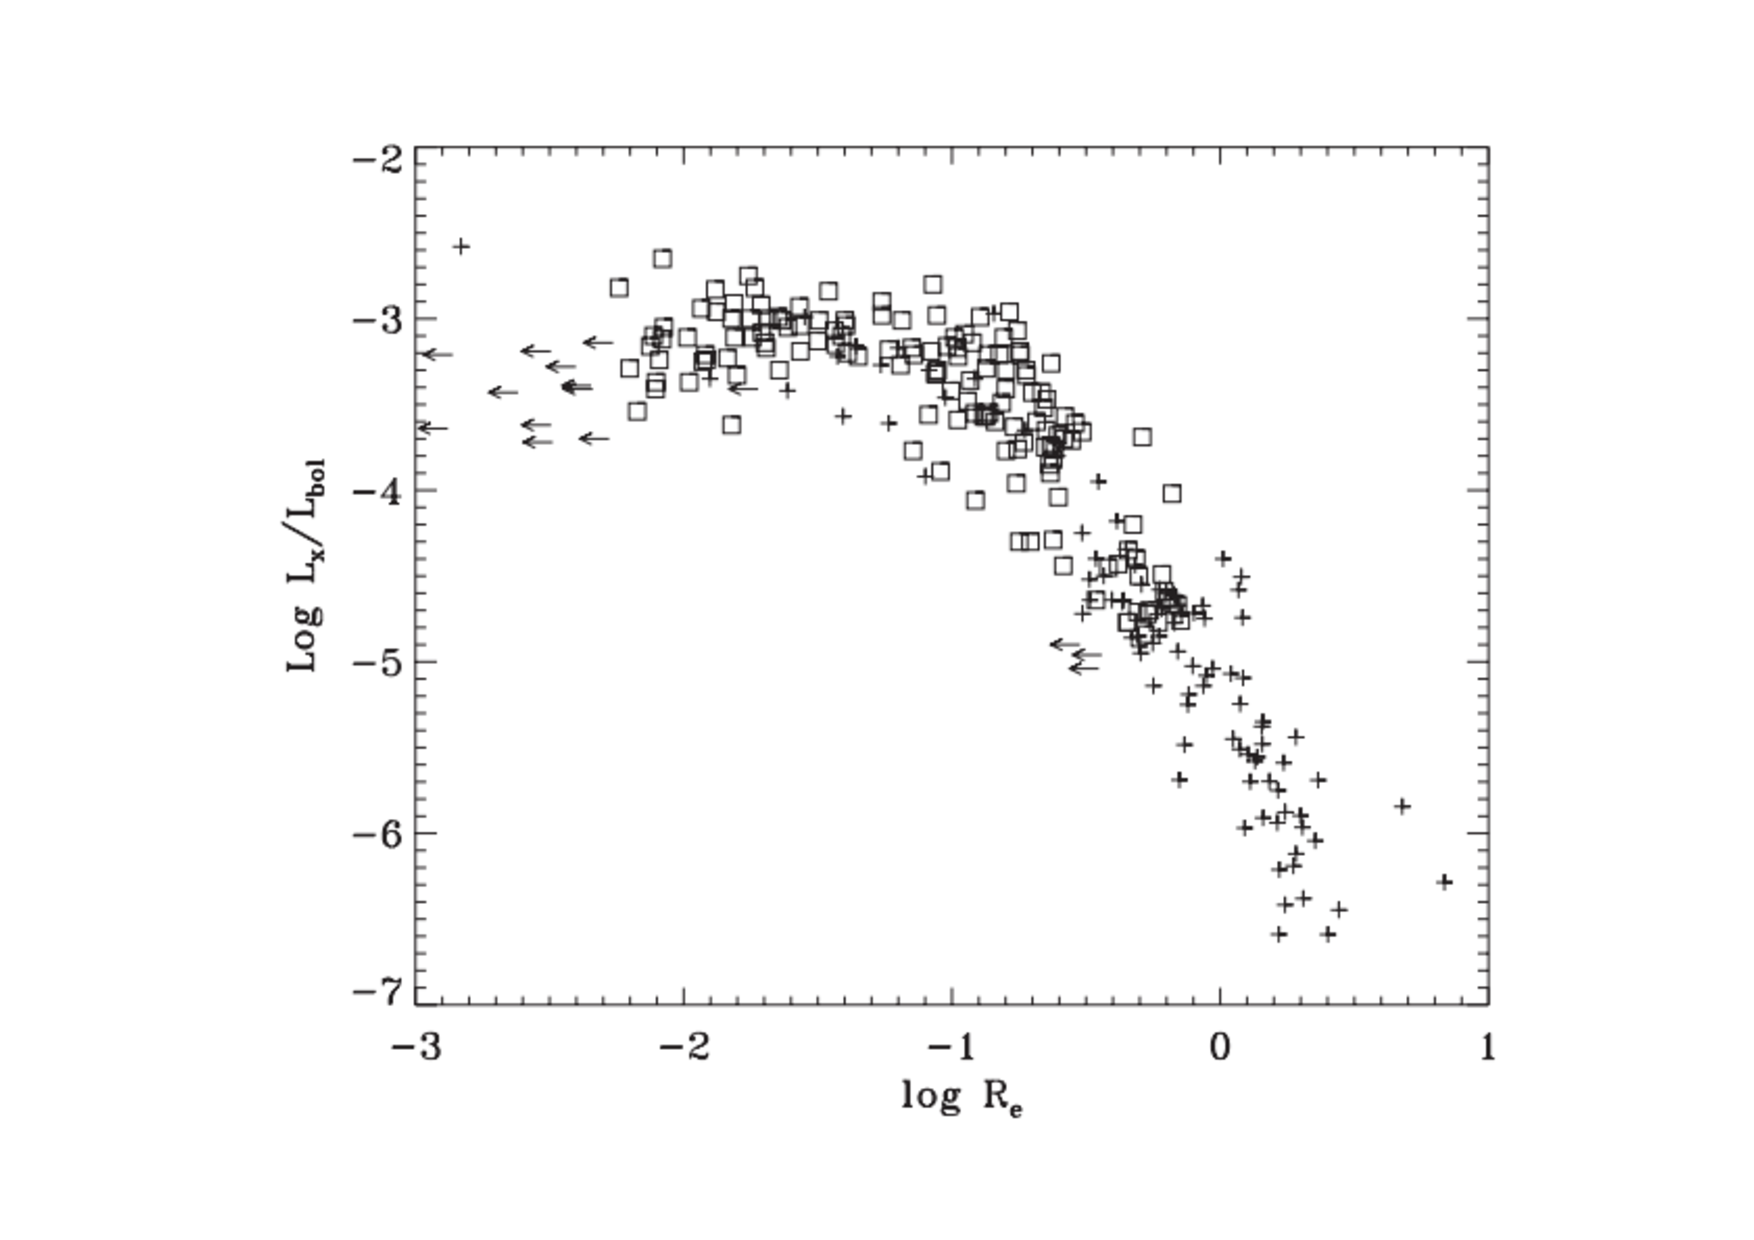
\includegraphics[scale=0.55]{Figures/2-Historical_overview/p03_fig_9.pdf}
    \caption[activity--rotation relationship from \citet{Pizzolato_etal_2003}]{Ratio of X-ray to bolometric luminosity as a function the empirically derived x-ray Rossby number for the \citet{Pizzolato_etal_2003} sample of stars. $v\sin i$ measurements are denoted by arrows. Image credit: \citet{Pizzolato_etal_2003}}
    \label{fig:pizzolato_etal_2003_plot}
\end{figure}

A later study of the activity--rotation relationship was conducted by \citet{Wright_etal_2011} which has a much bigger sample of 824 solar and late-type stars with X-ray luminosity and rotation periods. The goals of this paper were similar to that of \citet{Pizzolato_etal_2003}, namely to study the activity--rotation relationship and derive a new estimate of the convective turnover time. In this study they define the parameter $R_{x}$, which is simply the ratio of X-ray to bolometric luminosity. When considering their whole sample, they find a relationship between activity and rotation of the form: $R_{x} \propto R_{0}^{-2.18}$, which is slightly steeper than the canonical value of -2 seen in previous studies \citep{Pallavicini_etal_1981,Pizzolato_etal_2003}.

\begin{figure}[h]
    \centering
    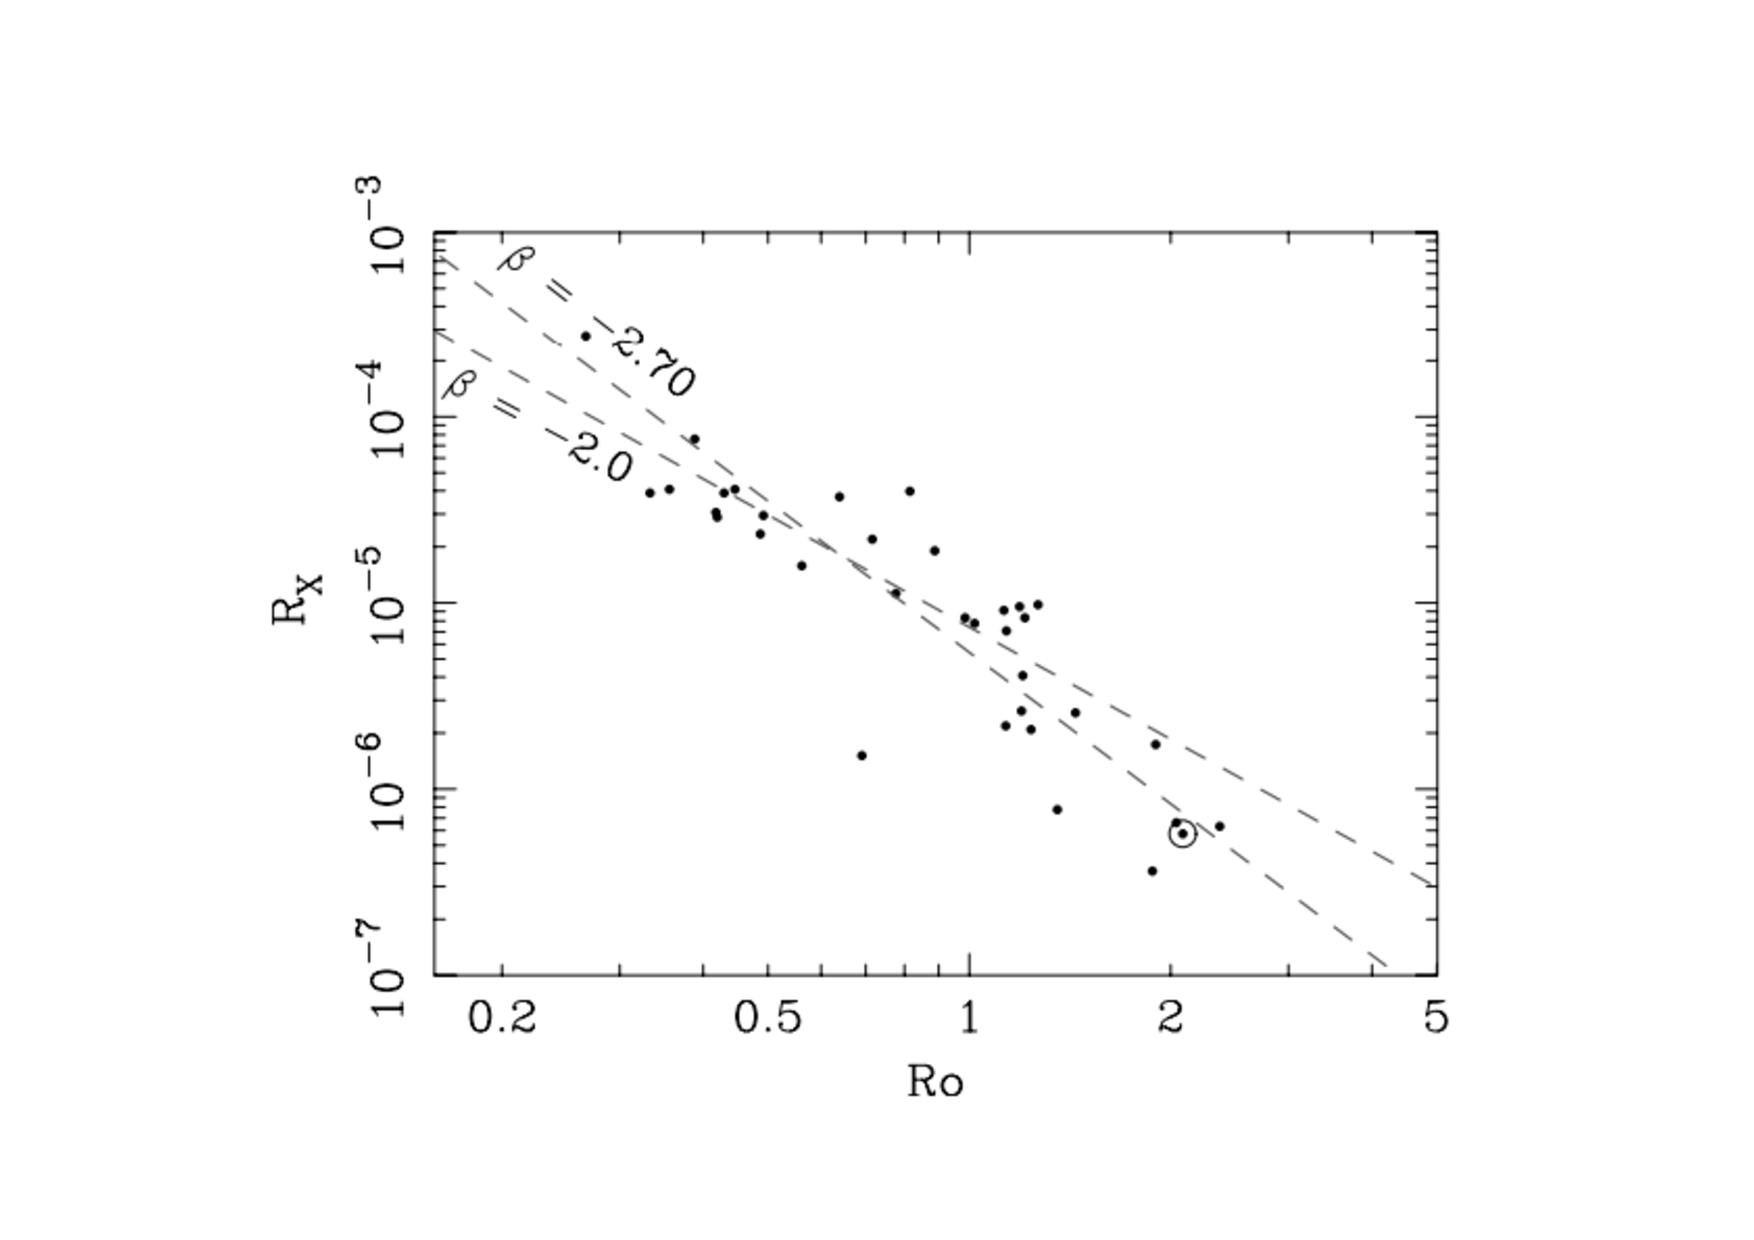
\includegraphics[scale=0.55]{Figures/2-Historical_overview/wright_etal_fig_3.pdf}
    \caption[Activity--rotation relationship for small, unbiased subset of \citet{Wright_etal_2011} data]{Small sample from \citet{Wright_etal_2011} that should be free from any detection bias in X-ray luminosity with $R_{x}$ plotted as a function of Rossby number. For this smaller sample, the best fitting relationship power law found has an exponent of $-2.70$, which is much steeper than the canonical value of $-2.0$. Image credit: \citet{Wright_etal_2011}}
    \label{fig:wright_etal_2011_plot}
\end{figure}

However, perhaps more importantly, they acknowledge that there are biases in their sample; at the largest $R_{0}$, it is likely that many of the faintest X-ray sources are not detected. Therefore they attempt to overcome these biases by compiling a smaller sample that should be unbiased. When they fit a power law to the smaller sample of 36 stars (as shown in Figure \ref{fig:wright_etal_2011_plot}), an exponent for the power law of $-2.70 \pm 0.13$ is found. This exponent value is much steeper than the value found for the whole sample but is in agreement with \citet{Gudel_etal_1997} and \citet{Feigelson_etal_2004} (which will be discussed in Section \ref{hist_xray_age_section}). This small, unbiased subset of data would suggest that there is a steepening of the activity--rotation relationship.

The most recent paper that concerned the activity--rotation relationship is by \citet{Metcalfe_etal_2016} which was motivated by the \citet{van_Saders_etal_2016} result and attempted to find a magnetic counterpart. The study compiled published values for the \Rprime indicator for the \citet{van_Saders_etal_2016} sample. They plotted the values found as a function of rotation period (seen in Figure \ref{fig:metcalfe_etal_2016_plot}) and compared their sample to G stars from the Mount Wilson survey. In \citet{Metcalfe_etal_2016}, a quantitative relationship is not fitted, however they do suggest that the Sun may be in a transitional evolutionary phase and may be a special case of stellar dynamo theory. They postulate that a change in the differential rotation is the underlying mechanism that disrupts the large scale organisation of magnetic field in solar-type stars and that at Rossby number of $\approx 2.0$, a shift in the magnetic topology causes the magnetic braking to operate with reduced efficiency. It is worth noting that the previous activity--rotation relationships all used the X-ray luminosity as the magnetic activity indicator and \citet{Metcalfe_etal_2016} is one of a few to study the chromospheric emission.

\begin{figure}
    \centering
    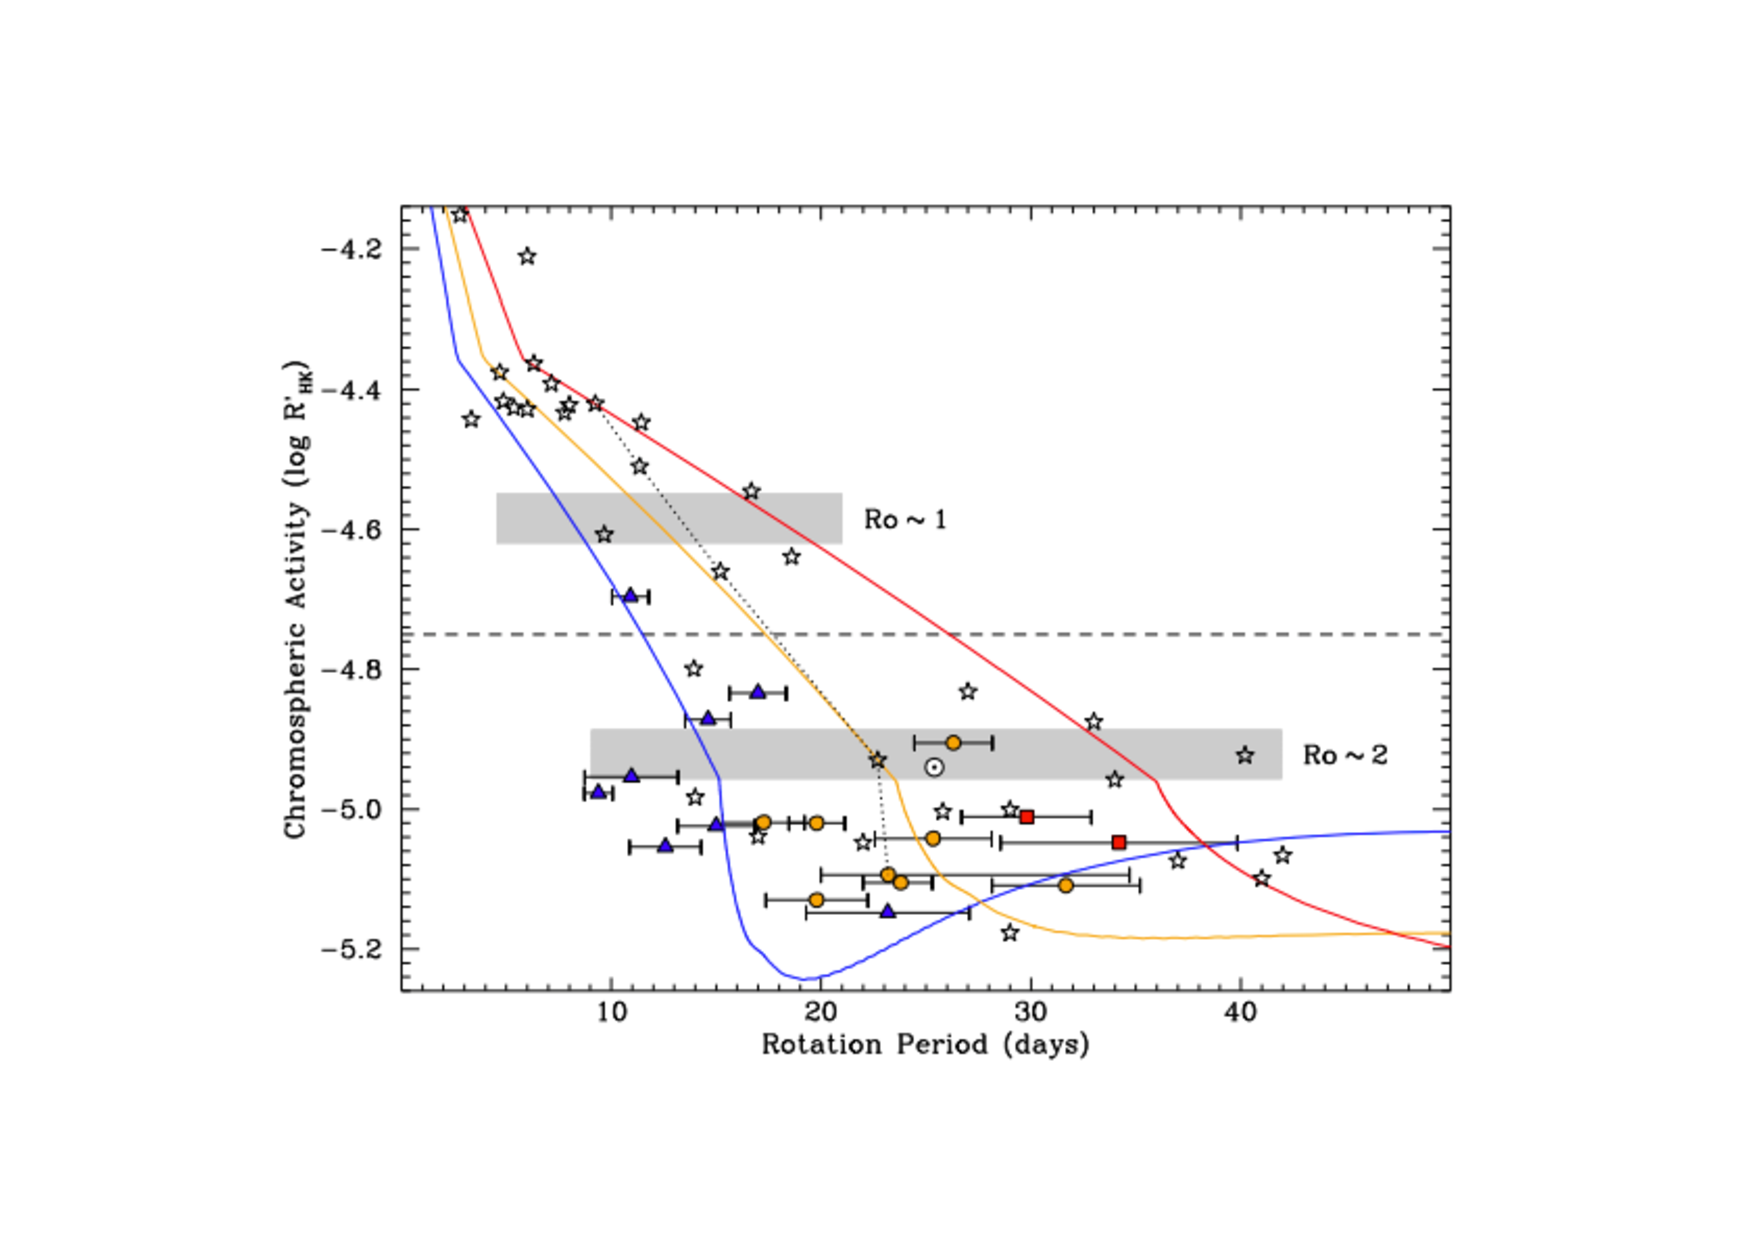
\includegraphics[scale=0.5]{Figures/2-Historical_overview/metcalfe_etal_2016_fig1.pdf}
    \caption[Chromospheric emission as a function of rotation period for sample of older stars]{Sample of stars from \citet{Metcalfe_etal_2016} with the \Rprime indicator plotted as a function of rotation period. Stars from the Mount Wilson survey are shown as star symbols. Rotational evolution models from \citet{van_Saders_etal_2016} are shown as lines. Image credit: \citet{Metcalfe_etal_2016}}
    \label{fig:metcalfe_etal_2016_plot}
\end{figure}

\section{Age--activity studies}
\label{Chp2_section_activity_age}
\subsection{Chromospheric emission - age relationship}

After the seminal paper by \citet{Skumanich_1972}, the method in which calcium emission was measured was changed by \citet{Noyes_etal_1984} who introduced the \Rprime indicator (as discussed in Section \ref{Chp1_atmosphere_chromosphere}). This is now the standard method of measuring the calcium emission in stars. Further studies investigated the age--activity relationship through chromospheric emission in the calcium lines including the following studies.

%Soderblom etal 1991
\citet{Soderblom_etal_1991} investigated the calcium emission - age relationship to determine firstly its existence as there was still debate at that time in the literature to whether the relationship was statistical or deterministic. Secondly, they also wanted to determine the nature of the relationship and expand on the three data points shown by \citet{Skumanich_1972}. Their sample of stars was compiled from several sources; the first being stars from clusters as these ages are well known through isochrone methods, but they also recognise that there are few clusters that were observable and older than the Hyades. The second source is stars in binary systems who have an evolved companion as the ages of these could be obtained through Str\"{o}mgren photometry. \citet{Soderblom_etal_1991} also included some evolved, single F dwarfs with known ages and stars whose relative age was known, for example, kinematic information placing stars within the old disk or halo populations.

From this sample of stars with ages and calcium emission they found that there was a deterministic relationship between the two parameters that followed this relationship - $R^{'}_{HK} \propto t^{-\frac{2}{3}}$. However, a problem arose when this power law was used to calculate ages for nearby solar-type stars; it was not consistent with a constant star formation rate, the ages calculated from this power law suggested that there was an excess of young stars ( $t < 1$ Gyr) in the solar neighbourhood. Therefore \citet{Soderblom_etal_1991} also computed a fit that was consistent with constant star formation rate and added a cubic dependence between the two parameters for stars younger than the solar age.

%Lachaume etal 1999
Another study in the literature concerning the calcium emission - age relationship was conducted by \citet{Lachaume_etal_1999} who aimed to calculate ages for a sample of stars using five different methods. They calibrated their calcium emission - age relationship using their sample of stars and the "best" age chosen from isochrone, metallicity or rotation. \citet{Lachaume_etal_1999} plotted these ages against literature values for the \Rprime indicator but found that the majority of the scatter was due to stars with $B - V$ values less than 0.6 therefore they exclude these stars from their sample. The calcium emission - age relationship they calibrate shows a decrease with age which then flattens when $log(R^{'}_{HK}) < -4.8$. Note that this relationship is not entirely independent as some ages have been taken from rotation measurements.

%MH08
Another important study was carried out by \citet{Mamajek_Hillenbrand_2008} (hereafter MH08) which compiled a large sample of solar-type dwarfs within the colour range of $0.5 < (B-V)_{0} < 0.9$. This study included an investigation of each of the components of the age--activity--rotation relation and populated the young end of the relationship for the first time. Their sample contained 167 main sequence and pre-main sequence stars taken from clusters and binary systems in the field with isochronal ages. They explored the age--activity relationship by plotting the mean value of the \Rprime indicator (as shown in Figure \ref{fig:MH08_age_activity_plot}) and found a quadratic fit was most appropriate in the range of their sample - $-5.1 < \log R^{'}_{HK} < -4.0$ and $6.7 < \log\tau < 9.9$ where $\tau$ is the stellar age in years. However, when inverting the relationship to have an expression in terms of stellar age, it was more accurate to have a trinomal function as shown in Equation \ref{Eq:MH_08_trinomal_eq}.

\begin{equation}
    \log R^{'}_{HK} = 8.94 - 4.849\log\tau + 0.624(\log\tau)^{2} - 0.028(\log\tau)^{3}
    \label{Eq:MH_08_trinomal_eq}
\end{equation}

\begin{figure}
    \centering
    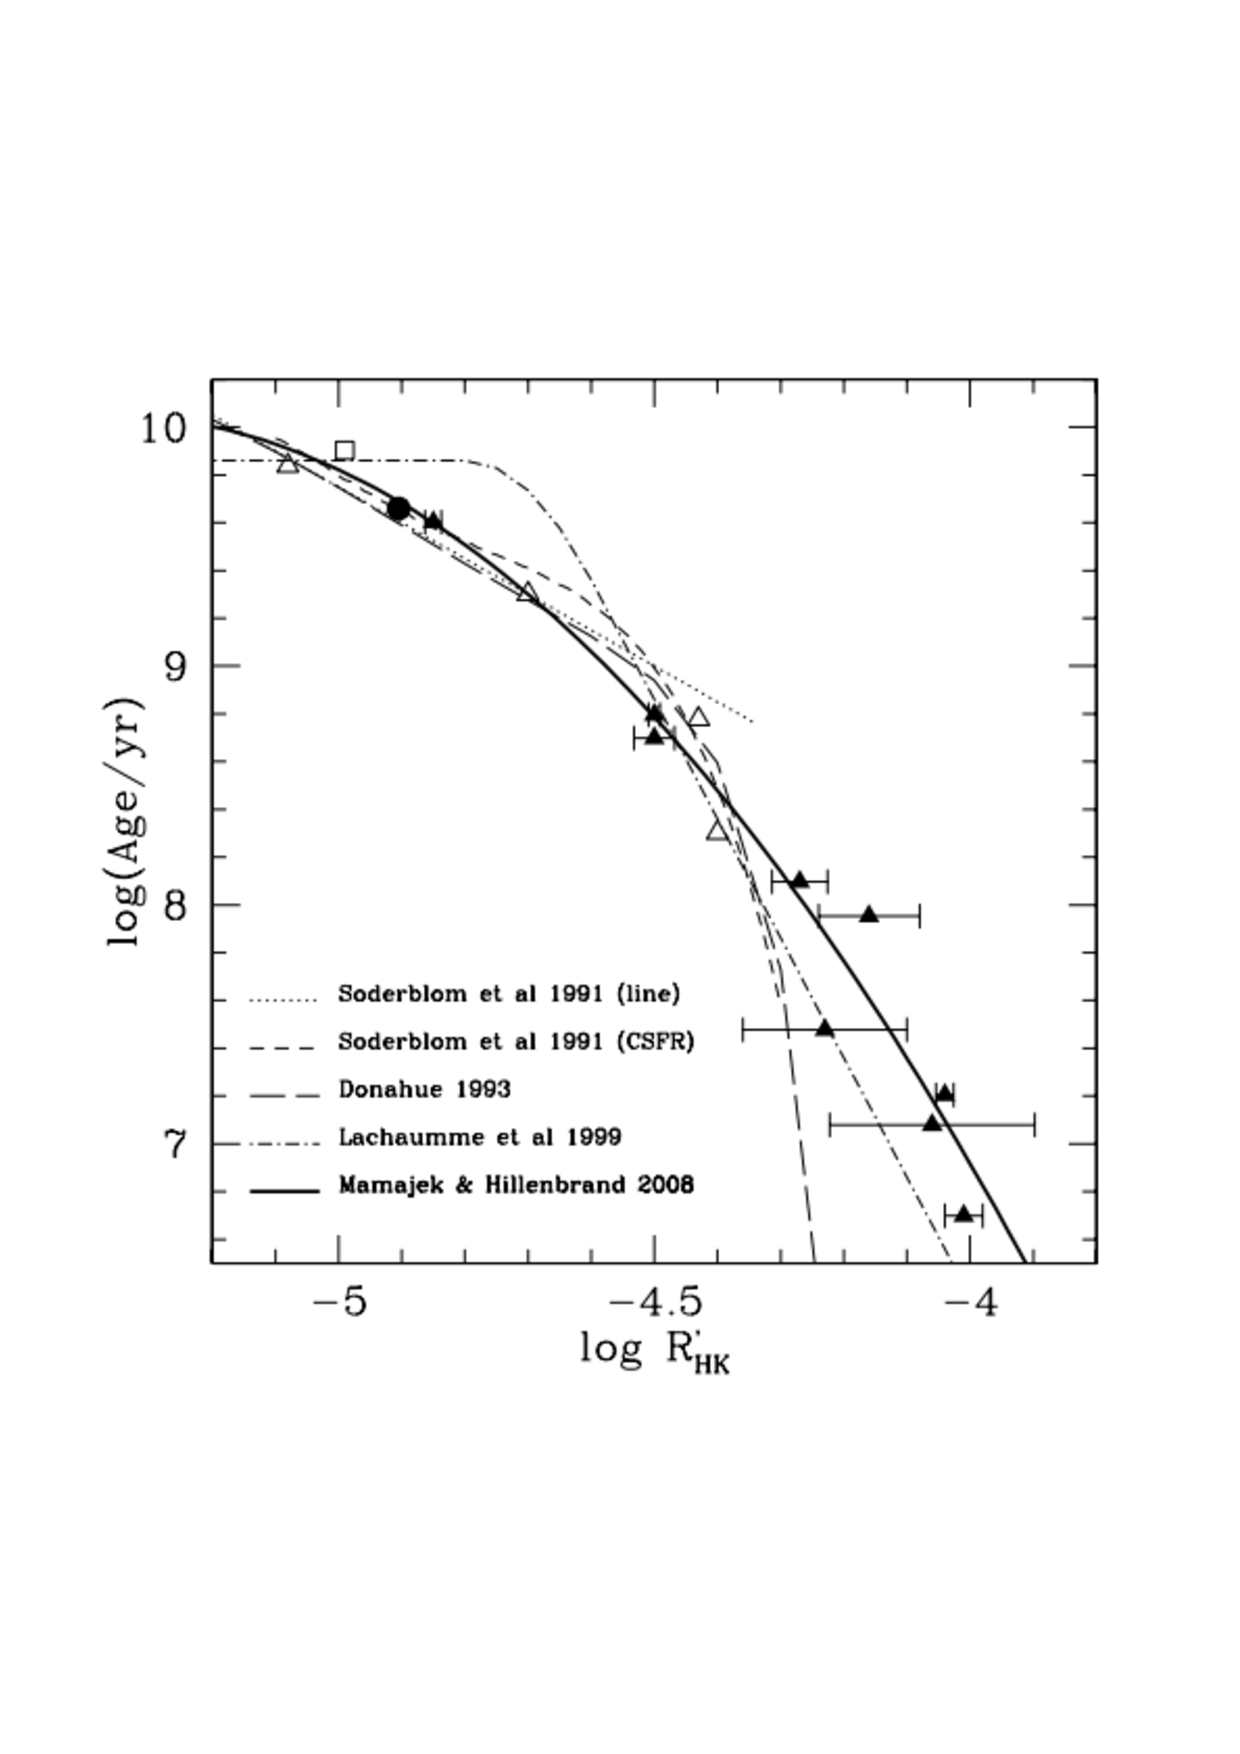
\includegraphics[scale=0.45]{Figures/2-Historical_overview/MH08_age_activity.pdf}
    \caption[age--activity plot from \citet{Mamajek_Hillenbrand_2008} using chromospheric emission]{age--activity plot from \citet{Mamajek_Hillenbrand_2008} that shows the \Rprime activity indicator as a function of stellar age for their sample. Previous age--activity relationships are plotted for reference in addition to their best fitting relationship. Image credit: \citet{Mamajek_Hillenbrand_2008}}
    \label{fig:MH08_age_activity_plot}
\end{figure}

Rotation periods were obtained for some of the MH08 sample, therefore the activity--rotation relationship was also investigated. The \Rprime indicator was plotted as a function of Rossby number  and three activity regions were found. For very active stars ($\log R^{'}_{HK} > -4.3$) little correlation was found between the two parameters, which is unsurprising as for very young stars there is a saturation of magnetic activity as seen in X-ray studies (e.g. \citealt{Jackson_etal_2012}). In the active regime ($-5.0 < \log R^{'}_{HK} < -4.3$), a very strong anti-correlation is found with Pearson coefficient (r) of -0.94. Lastly, in the inactive regime ($\log R^{'}_{HK} < -5.0$), very weak correlation is observed; note this is based on a small number of data points that seem to have a fairly large spread in Rossby number. From these rotation periods the study was also able to update the coefficients for the \citet{Barnes_2007} gyrochronology relationship.

MH08 also investigated the \Rprime indicator as a function of colour among binaries and kinematic groups to see if there is a mass dependency as these systems can be assumed to be the same age but different masses. For the 24 binary pairs a range of slopes between the \Rprime indicator and colour were found, both positive and negative. For a similar plot of the \Rprime indicator and colour for the kinematic groups there were no unique slopes applicable to all activity levels. In this plot, younger groups such as the Pleiades showed steep positive slopes which were $\approx 2\sigma$ steeper than the slope for Hyades. The oldest cluster displayed the most negative slope which may suggest that the slope ($\Delta\log R^{'}_{HK} / \Delta(B- V)$) may flatten as a function of age.

%Pace 2013
\citet{Pace_2013} called the age--activity relationship into question, particularly when using chromospheric emission from the \caII spectral lines. There was some evidence from open clusters that the chromospheric activity in stars with ages of 1.5 Gyr had similar activity levels to the solar value \citep{Pace_Pasquini_2004}. Therefore this study aimed to calibrate the age activity relationship, particularly for ages older than one gigayear. This was achieved by considering field stars with literature values for the \Rprime indicator and isochronal ages from the Geneva-Copenhagen survey of solar neighbourhood (GCS). Only stars with sufficiently precise ages were selected for the study, errors on the age had to be less than 2 Gyr.

The \Rprime indicator was plotted for the final sample of 1744 field dwarfs as a function of their stellar age as shown in Figure \ref{fig:pace_2013_plot}. This plot shows an L-shaped age--activity relationship which seems to suggest that the decay of chromospheric activity stops a a relatively young age. The age at which the chromospheric activity seems to stop its evolution is approximately 3 Gyr from the sample of field stars, however, due to the errors associated with the stellar age it may actually stop sooner than this. It is also worth noting that as the age of sample increases, the effective temperature of the stars in the sample decreases thus indicating that there may be biases in the sample. If the evolution of the chromospheric activity does indeed stop at a relatively early age then this would hinder the use of the parameter as an age indicator.

\citet{Pace_2013} also considered a sample of open clusters and found that there was a difference in the trend of the \Rprime indicator as a function of effective temperature depending on whether it was an active or inactive cluster. Young clusters tended to have a slight increase of the \Rprime with decreasing effective temperature. Older clusters had a more complicated pattern of the \Rprime indicator with effective temperature. The difference in age between the oldest active cluster and youngest inactive cluster was just 50 Myr. This was suggested to be due to a sudden drop in chromospheric activity however there was some doubt over the dependency of the oldest active cluster.

\begin{figure}
    \centering
    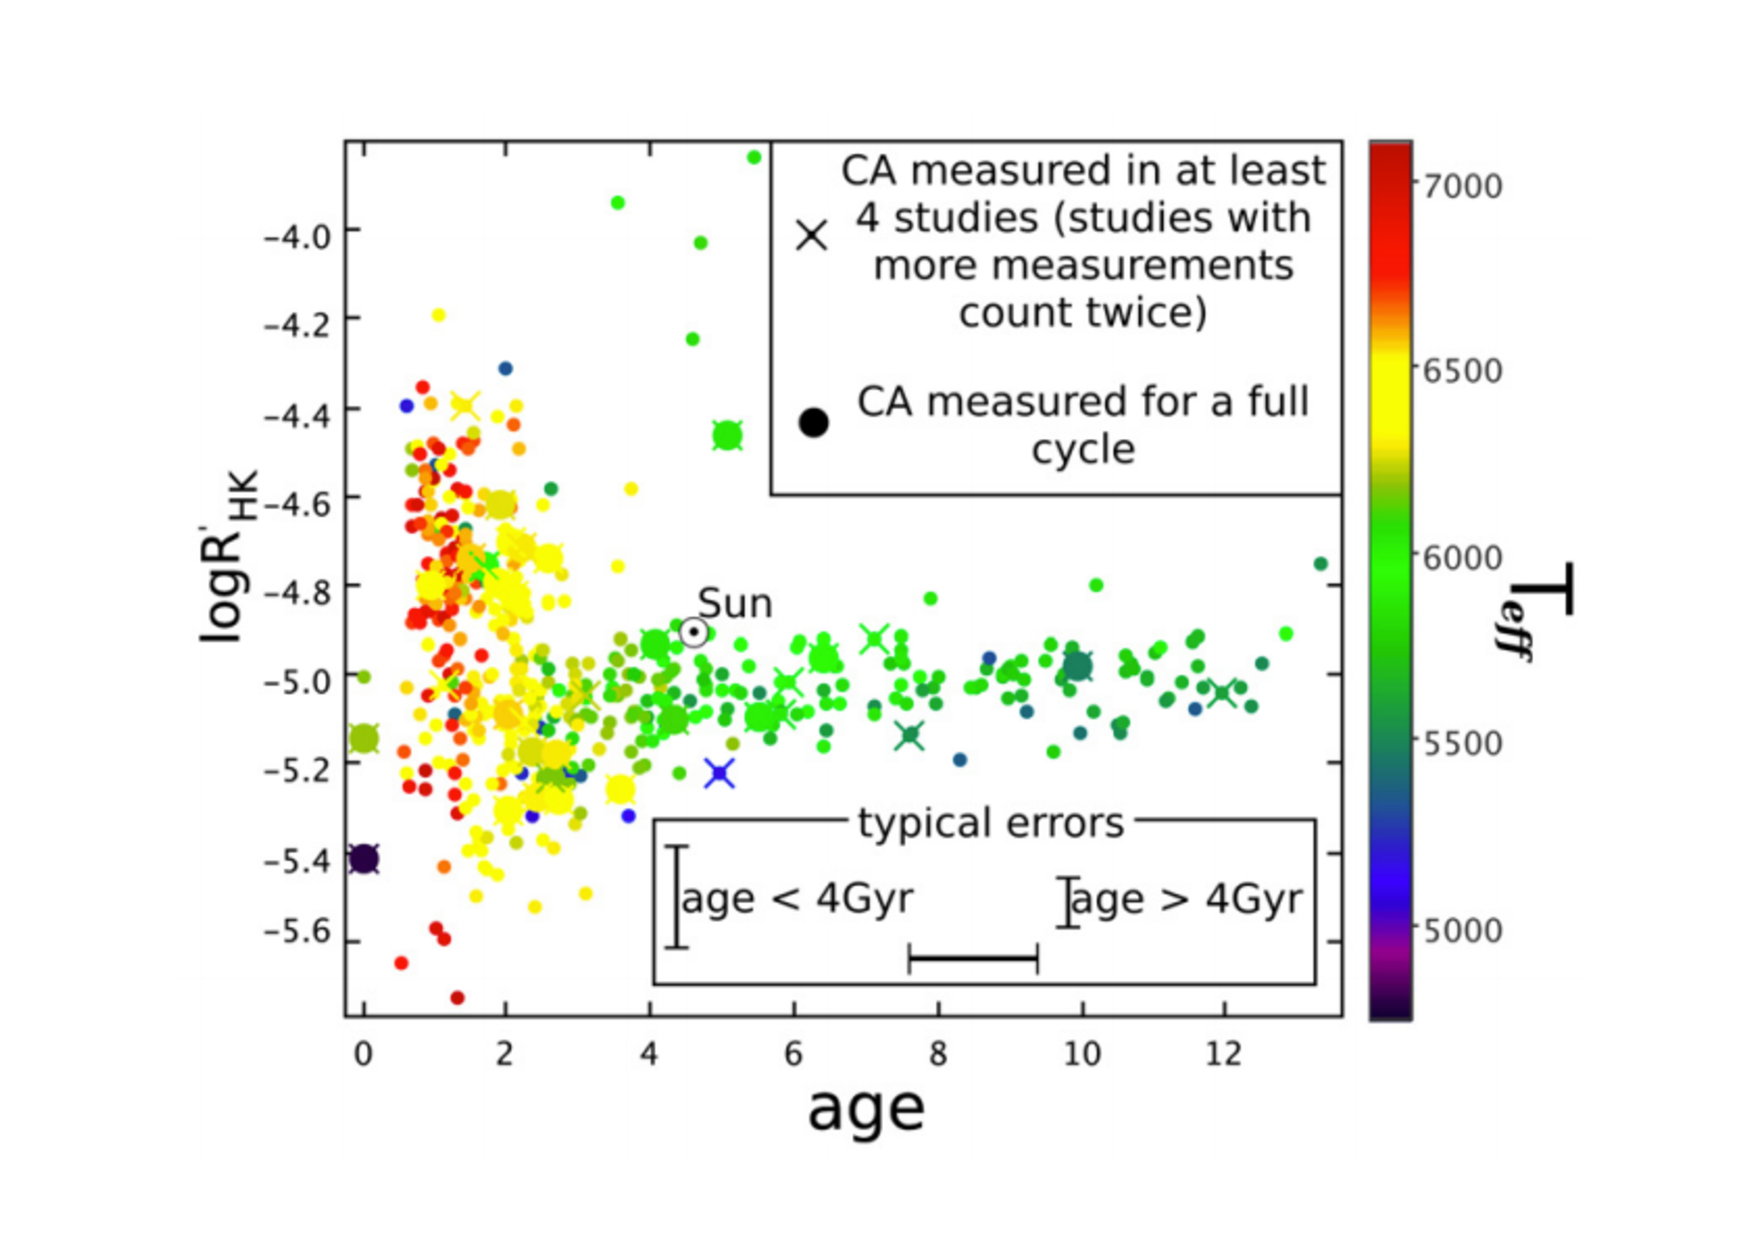
\includegraphics[scale=0.4]{Figures/2-Historical_overview/pace_2013.pdf}
    \caption[\citet{Pace_2013} age--activity relationship]{\citet{Pace_2013} plot of calcium chromospheric emission as a function of stellar age for the sample of field dwarfs with isochronal ages. Data points are coloured according to their effective temperature. Image credit: \citet{Pace_2013}}
    \label{fig:pace_2013_plot}
\end{figure}

%LO_etal_2016 (AMMAR)
While the age--activity relationship was called into question by \citet{Pace_2013}, this lead others to consider the potential issues with using the \Rprime indicator as an activity indicator. The work by \citet{Lorenzo_Oliveira_etal_2016} is an example of such a study, they analysed the presence of mass and metallicity biases that are implicit in conventional methods of selecting solar-type stars with precise isochronal ages such as the method in \citet{Pace_2013}. They argue that in order to obtain precise isochronal ages, most stars will be more massive than the Sun as a sizeable detachment from the ZAMS is needed to calculate a reliable age. Furthermore, such a sample will have a large range of metallicities and due to the age--metallicity relationship younger stars tend to be more metal rich. This has consequences for the chromospheric activity measured in these stars as they have deeper \caII profiles thus mimicking more subdued chromospheric activity. Younger stars in these types of samples also tend to be more massive (due to the necessary detachment from ZAMS for a reliable age), such stars have a decreased convective efficiency and will appear less active. Both of these selection effects combine to lower the chromospheric activity of the younger population of a sample. Conversely, older stars tend to be less massive and appear more active to to an increase in their convective efficiency. These older stars also tend to be metal-poor which will lead to shallower \caII profiles and mimic higher levels of chromospheric activity. The net result of such biases in a large sample will blur the range of the \Rprime indicator between young and old stars thus masking the true structure of the age--activity relationship.

In order to study this in more detail \citet{Lorenzo_Oliveira_etal_2016} collected a sample of field stars and open cluster members and derived an age--mass-metallicity-activity relation (hereafter AMMAR). The AMMAR is shown in Equation \ref{Eq:AMMAR} where $\beta_{0}$ = -56.01, $\beta_{1}$ = -25.81, $\beta_{2}$ = -0.44, $\beta_{3}$ = -1.26 and $\beta_{4}$ = -2.53. They compared chromospheric ages from the MH08 relationship and their AMMAR to asteroseismic ages. The chromospheric ages calculated from their AMMAR showed excellent agreement with the asteroseismic ages. However, the chromospheric ages from the MH08 relation showed a trend in the difference between it and the asteroseismic age with metallicity. This further confirmed that the metallicity of a star can affect the chromospheric emission measured in \caII spectral lines and that it should be accounted for.

\begin{equation}
    \log(t) = \beta_{0} + \beta_{1}\log(R^{'}_{HK}) + \beta_{2}[Fe/H] + \beta_{3}\log(M/M_{\odot}) + \beta_{4}\log(R^{'}_{HK})^{2}
    \label{Eq:AMMAR}
\end{equation}

\citet{Lorenzo_Oliveira_etal_2016} were also able to reproduce the L-shaped age--activity relationship shown in \citet{Pace_2013} by selecting stars from GCS and using the same selection rules. They calculated the \Rprime indicator using their AMMAR and plotted the mean value and its dispersion as a function of age. They found that there was a constant metallicity dispersion ($\approx 2\sigma$) along the age domain which is understood to be an additional source of scatter in the age--activity relationship. Furthermore, the sample is increasingly bias towards higher masses at young ages which can also be seen in the plot from \citet{Pace_2013} in Figure \ref{fig:pace_2013_plot}.

%Lorenzo-Oliveira etal 2018
Considering the evidence of mass and metallicity effects on the \Rprime indicator, it seems that care must be taken when considering large sample of stars. In order to minimise these effects, careful selection criteria must be enforced to the sample. An example of such a study was undertaken by \citet{Lorenzo_Oliveira_etal_2018}, where they consider a sample of solar twins with isochronal ages. Spectroscopic binaries and stars in a binary systems with a companion closer than 4" were removed from sample as close companions may exchange angular momentum with the solar twin, therefore altering the evolution of the stellar angular momentum.

\begin{figure}
    \centering
    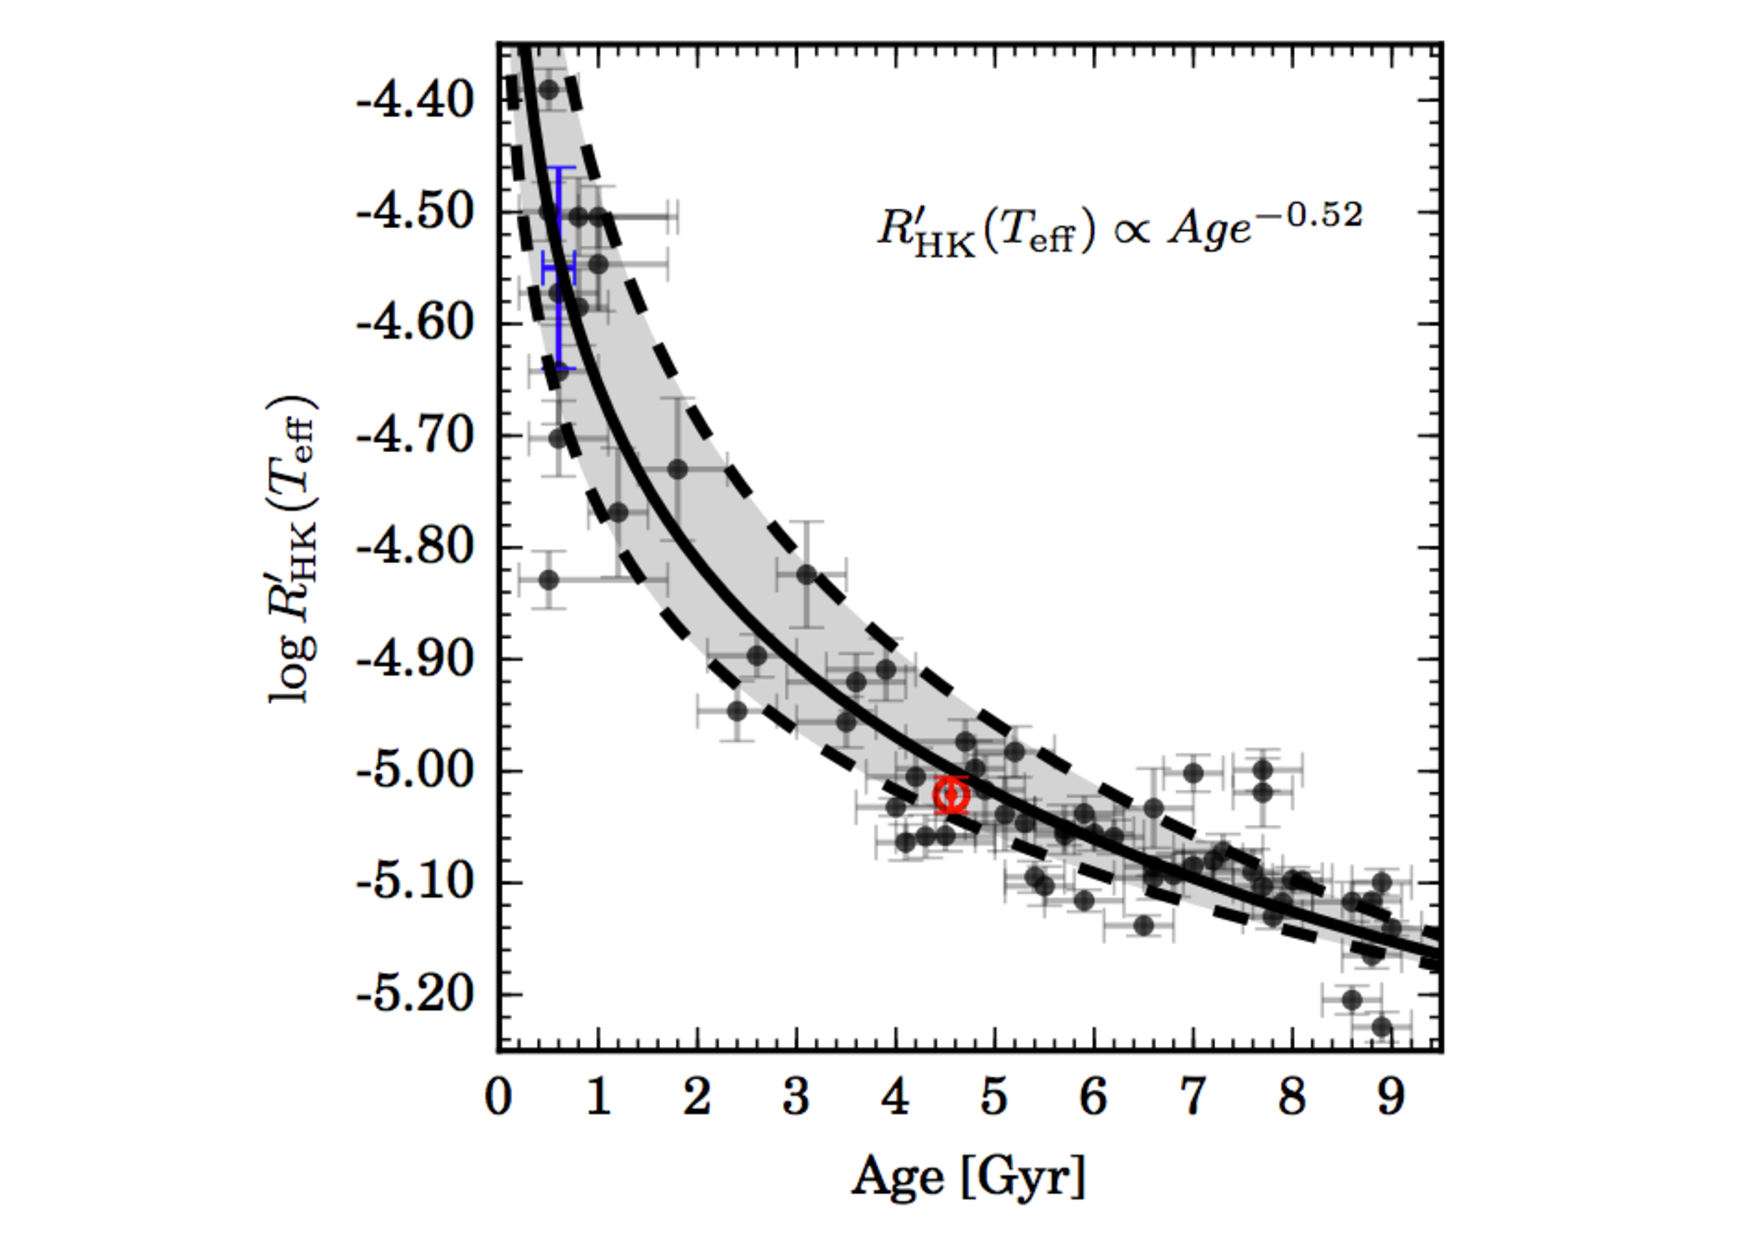
\includegraphics[scale=0.45]{Figures/2-Historical_overview/LO_etal_18_age_activity_plot.pdf}
    \caption[\Rprime - age relationship for sample of solar twins]{The \Rprime indicator (calibrated to effective temperature) plotted as a function of isochronal age for a sample of solar twins. The Sun is shown as a red symbol and stars younger than a gigayear are represented by a single cluster (blue data point). The black line is the best fitting relationship which is given by Equation \ref{Eq:LO_etal_18_law}. The shaded region is the 2$\sigma$ activity variability prediction band. Image credit: \citet{Lorenzo_Oliveira_etal_2018}}
    \label{fig:LO_etal_18_plot}
\end{figure}

The S index was calculated for each star using spectra from HARPS and calibrated to the Mount Wilson S index (\Smw). There are a number of reasons why the S index must be calibrated to the Mount Wilson index, firstly due to the calculation of the \Rprime indicator which is based off the Mount Wilson value. Secondly, the value of the S index is dependent on the throughput of the spectrometer thus in order to have consistent values for the S index it is transformed into the Mount Wilson value. Once the \Smw value had been determined for the sample, this could then be converted into the \Rprime indicator. However, \citet{Lorenzo_Oliveira_etal_2018} calibrated the correction factor $C_{cf}$ as a function of effective temperature and claimed to improve the method used to calculate the \Rprime indicator.

\citet{Lorenzo_Oliveira_etal_2018} plotted their \Rprime values (calibrated to effective temperature) as a function of the isochronal age which is shown in Figure \ref{fig:LO_etal_18_plot}. The best fitting relationship (Equation \ref{Eq:LO_etal_18_law} where Age is in Gyr) shows that for this sample of solar twins, the decay of magnetic activity with time is very close to that of the Skumanich Law. More importantly, it confirms that the age--activity relationship remains statistically significant after solar age for solar twins.

\begin{equation}
    R^{'}_{HK}(T_{eff}) \propto Age^{-0.52}
    \label{Eq:LO_etal_18_law}
\end{equation}

\subsection{Coronal activity - age relationship}
\label{hist_xray_age_section}
We know that magnetic activity is also displayed in the corona and that the X-ray luminosity is a good magnetic activity indicator. Therefore, it is no surprise that there have also been attempts to calibrate an age--activity relationship by using the X-ray luminosity as a magnetic activity indicator. One of the earliest attempts was by \citet{Maggio_etal_1987} who used a survey of late-F and G type stars from the Einstein telescope to investigate a volume-limited sample. As part of this investigation, they plotted the X-ray luminosity as a function of age. Note that the ages used in this study were either cluster ages or individual ages based on lithium abundances. They found that their sample followed a relationship of the form: $L_{x} \propto t^{-1.5}$. However, this did include upper limits for X-ray luminosities and lower boundaries for stellar ages.

%Gudel etal 1997
A later study by \citet{Gudel_etal_1997} investigated the dependence of coronal temperature and emission measure on age and rotation period using a sample of nine solar-like G stars with ages from 70 Myr to 9 Gyr and data from the ASCA and ROSAT X-ray satellites. Previous X-ray studies had indicated that the corona of active stars tended to be hotter than low activity analogues \citep{Schmitt_etal_1995}. \citet{Gudel_etal_1997} confirm this with their sample of stars, finding a dependence between X-ray luminosity and the value of the hotter temperature component of the form: $L_{x} \propto T_{hot}^{4}$. this is interpreted as a decrease in the efficiency of the high temperature coronal heating mechanism as a function of age. Ages were also collected for their sample of G type stars from clusters/moving groups, rotational and isochronal ages. They found that the best fitting relationship between the X-ray luminosity and stellar age followed a power law with an exponent of $-1.5$, in agreement with the findings of \citet{Maggio_etal_1987}.

%Feigelson etal 2004
A different approach was taken by \citet{Feigelson_etal_2004} who utilised the Chandra deep field - North (CDF-N) which probes a region of the sky to a very low X-ray limit of $3 x 10^{-17}$ cm$^{-2}$ ergs s$^{-1}$ in the soft band (0.5 - 2 keV). \citet{Feigelson_etal_2004} used the $\approx$ 3\% of the sample that were low mass stars resulting in 11 stars. While individual ages were not known for these stars, limits to the ages could be determined. The stars in the sample were not sufficiently high above the galactic plane to be likely members of the thick disc or halo, both of which are known to be very old. Therefore, the stars in the sample must belong to the thin disk , thus setting an upper limit for their age of 11 $\pm$ 1 Gyr.

Instead of plotting X-ray luminosity as a function of age since individual ages were not available, the observed X-ray distribution of the sample was compared to predicted populations assuming different magnetic activity decay laws of the form: $L_{x} \propto t^{\alpha\beta}$ where $\alpha$ represents the exponent of the rotational spin-down law (Equation \ref{Eq:general_rotation_age}) and $\beta$ is the exponent of the activity--rotation law (Equation \ref{Eq:general_activity_rotation}). This approach was only feasible due to the nature of the CDF-N, it is complete in both X-ray population and the identification of stellar counterparts (within the flux limits). \citet{Feigelson_etal_2004} find that a value for the decay law exponent of $\alpha\beta = -2$ provides an excellent fit to the data but due to the small sample size and systematics they also cannot rule out an exponent value of $\alpha\beta = -1$ which is the expected value from other studies of age--rotation and activity--rotation relationships.

%Giardino etal 2008
\citet{Giardino_etal_2008} studied the X-ray luminosities for members of NGC 752, a 1.9 Gyr old cluster. Clusters with this approximate age are useful as they bridge the gap in between the Hyades and the Sun where most of the decrease in X-ray luminosity occurs. Seven data points for NGC 752 were obtained and plotted alongside data for other clusters and the Sun. The median X-ray luminosity of NGC 752 showed good agreement with the decay magnetic activity trend and was consistent with an exponent of $\alpha\beta \sim -1.5$. Again, these results are in agreement with \citet{Maggio_etal_1987} and \citet{Feigelson_etal_2004}.

%Jackson etal 2012
Probably the largest study of the X-ray luminosity-age relationship to date was conducted by \citet{Jackson_etal_2012} that studied a large sample of stars in open clusters. They selected 717 stars from 13 open clusters and aimed to study in particular the saturated regime of the activity--age relationship and the implications for exoplanets. Their sample had a (B-V) colour range of 0.29 to 1.41 which consists of F, G and K stars. Upper limit results for $L_{x}$, giant stars and flare stars were excluded from the analysis. The sample was filtered into colour bins as a proxy for mass since the decay of magnetic activity is expected to depend on this parameter.

\begin{figure}[t]
    \centering
    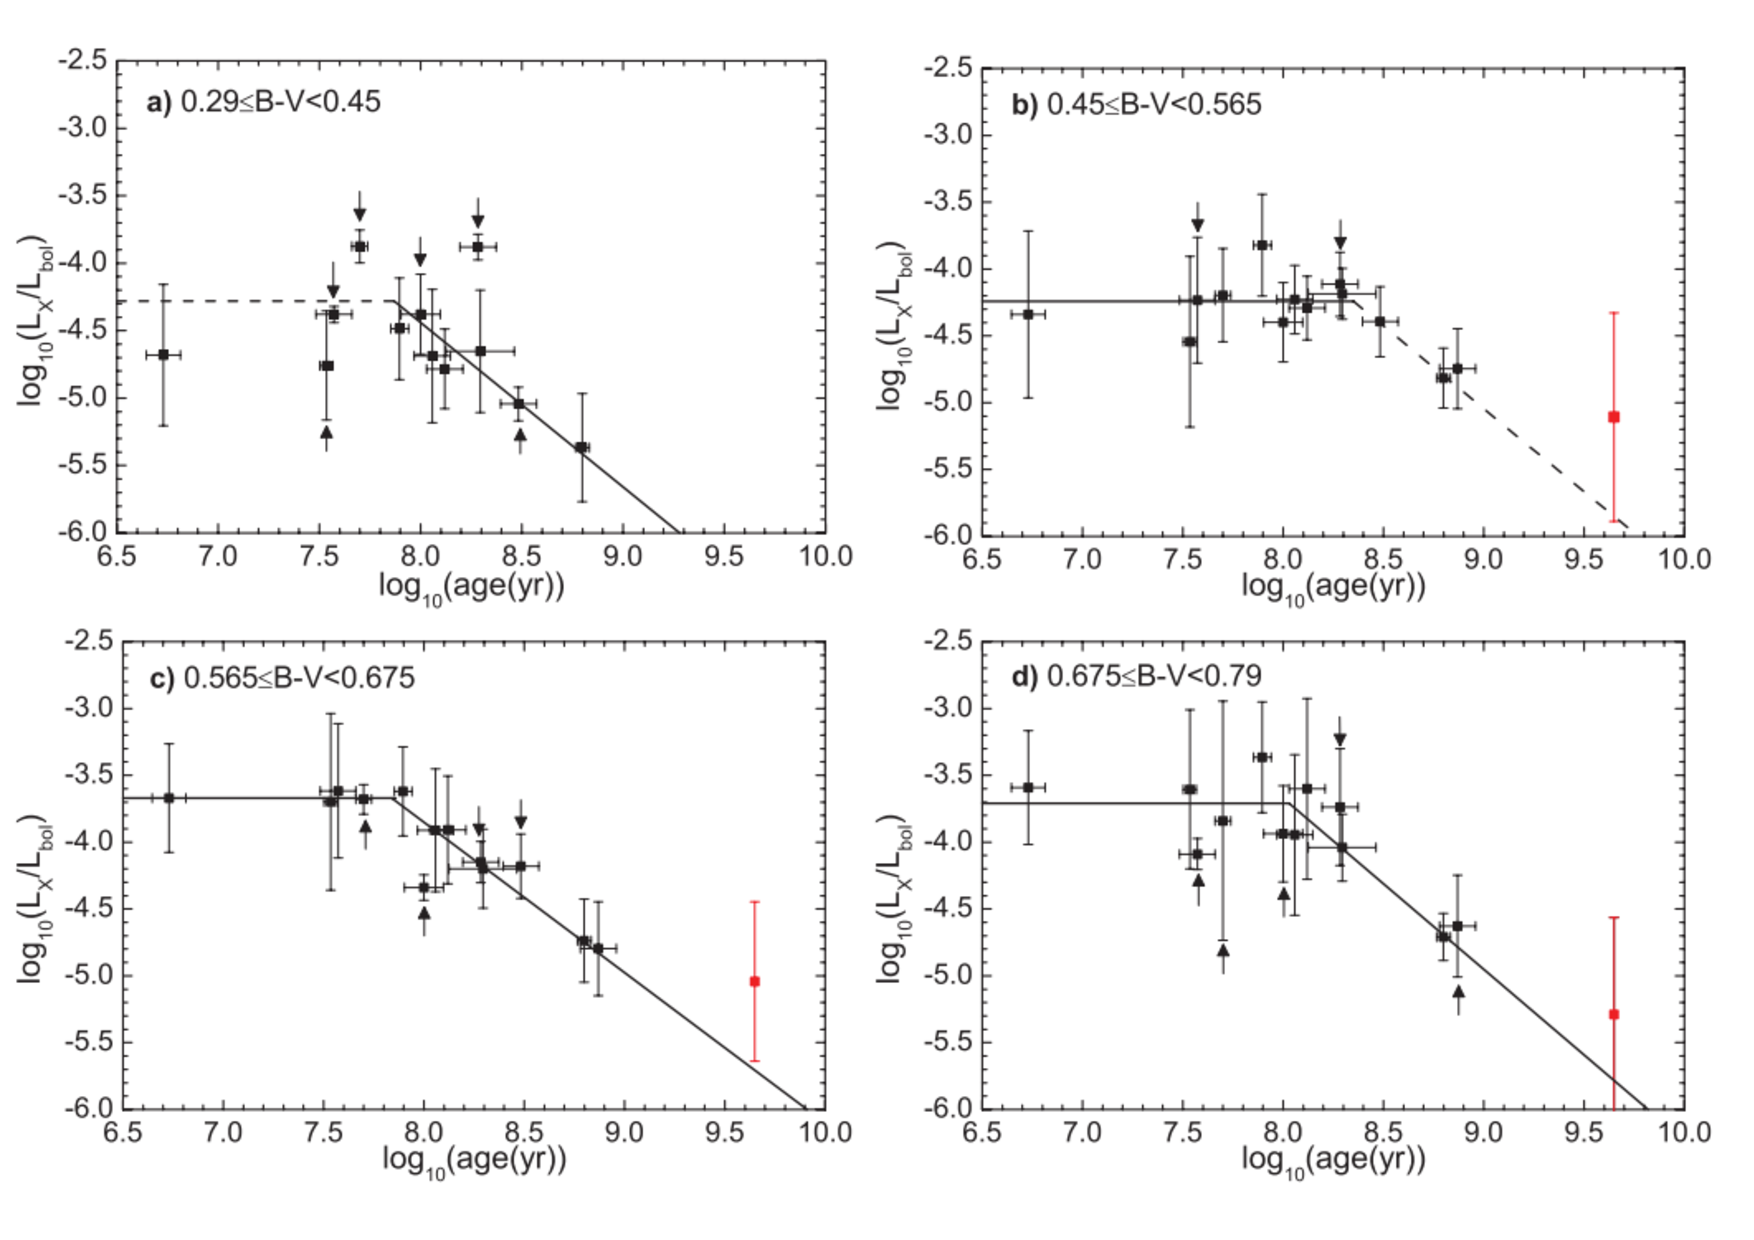
\includegraphics[scale=0.45]{Figures/2-Historical_overview/jackson_etal_2012_part.pdf}
    \caption[\citet{Jackson_etal_2012} X-ray luminosity - age relationship for sample of clusters]{Plot of X-ray luminosity as a function of stellar age for cluster data. Each subplot shows the relationship in a particular mass bin as defined by the (B-V) colour. Solid lines indicate best-fitting relationships, while dashed lines show more uncertain fits. Red data point indicates the field sample from \citet{Pizzolato_etal_2003} for reference. Image credit: \citet{Jackson_etal_2012}}
    \label{fig:jackson_etal_2012_plot}
\end{figure}

While the previous studies discussed concentrated on measuring the rate of decay of magnetic activity with time, this study also focused on measuring the saturated X-ray emission at very young ages. This is clearly seen in the activity--rotation relationships (see Section \ref{Chp2_activity-rotation_lit_review}), where at rotation periods shorter than $\sim 1-2$ days the trend of increasing X-ray luminosity with decreasing rotation period stops and the X-ray luminosity is constant for very fast rotators. At these extremely fast rotation rates, it is thought that the coronal emission is at the physical maximum, i.e. the star has no more available surface area to accommodate more active regions \citep{Jardine_Unruh_1999}.

In \citet{Jackson_etal_2012}, a broken power law was fitted to the cluster data in each (B-V) bin as shown in Figure \ref{fig:jackson_etal_2012_plot}. In the saturated regime, the gradient was constrained to be zero but in the unsaturated regime this was allowed to vary. Their fitted relationships suggested that there was a decrease in the saturated X-ray luminosity as (B-V) value increased. The resulting slopes for each (B-V) bin range from $-1.09$ to $-1.40$ with a typical error of $\pm 0.2$ dex. However, no obvious trends for the change in slope with spectral type were found.

\section{Current knowledge and limitations}
As demonstrated in this section, much progress has been made with the age--activity--rotation relationships since the early work of \citet{Kraft_1967} and \citet{Skumanich_1972}. In regards to gyrochronology, larger data sets have become available but the challenge has become the interpretation of such large data sets, especially understanding the biases that may be present in such samples \citep{van_Saders_etal_2019}. This issue with calibrating the gyrochronology relationship to the solar age (and beyond) is that the rotation periods are much longer and therefore require a much longer baseline for observations. In addition to this, determining rotation periods from light curve variation requires the presence of starspots, indicating fairly high levels of activity. Since the magnetic activity of the star is also expected to decrease with age, the amount of starspots would be expected to decrease along with their associated light curve amplitude. Perhaps in the case of old main sequence stars, it would be better to consider other parameters such as magnetic activity indicators that are not reliant on the presence of starspots.

While most activity--rotation studies find that the value for the power law exponent is -2.0, there is some doubt cast over this value as \citet{Wright_etal_2011} found a much steeper value for a smaller, unbiased sample of stars. \citet{Metcalfe_etal_2016} also questioned the nature of the activity--rotation relationship by postulating that the Sun is in a transitional evolutionary phase. There is still work to be done regarding the activity--rotation relationship but it requires a knowledge of the potential biases present, especially concerning the completeness of low-activity samples as demonstrated in \citet{Wright_etal_2011}.

There have been many studies on the chromospheric activity--age relationship, particularly in recent years where there has been a debate over it's suitability as an age indicator. Attempts have been made to extend the relationship to older ages (i.e. older than a gigayear) but with varying success - \citet{Pace_2013} found an L-shaped activity--age diagram whereas \citet{Lorenzo_Oliveira_etal_2016} argued that this was due to subtle dependencies on mass and metallicity. Claims have been made that for solar twins at least, the relationship is valid to at least solar age \citep{Lorenzo_Oliveira_etal_2018}. However, the relationship has not been studied with asteroseismic ages, most studies in recent years have used isochronal ages.

Lastly, while there have only been a handful of studies concerning the X-ray luminosity-age relationship, it is expected to follow a relationship of the form: $L_{x} \propto t^{-1}$ from previous studies concerning gyrochronology and activity--rotation relationships. \citet{Jackson_etal_2012} found for a sample of stars from open clusters that the value for the exponent of this relationship tended to be slightly larger than the expected value of $-1.0$. While efforts have been made to extend the chromospheric-age relationship to ages older than a gigayear using isochronal ages, no attempts have been made to extend to attempt this for the X-ray luminosity-age relationship.

The focus of the work presented in this thesis is to try and understand the age--activity--rotation relationship beyond a gigayear by considering ages determined from asteroseismology. In Chapter \ref{Chapter3} I present the first study to study the X-ray luminosity-age relationship beyond a gigayear in detail. With motivation from the X-ray luminosity-age study, Chapter \ref{Chapter4} presents a similar study using chromospheric emission as the magnetic activity indicator. Finally, Chapter \ref{Chapter5} will attempt to put the results found from the age--activity relationships into context by considering rotation periods.